\documentclass[11pt,a4paper]{article}
\usepackage{amsmath,amssymb,graphicx,geometry,booktabs,hyperref,longtable}
\usepackage{amsthm}
\newtheorem{proposition}{Proposition}
\usepackage{setspace}
\usepackage{siunitx}
\onehalfspacing
\emergencystretch=3em
\geometry{margin=1in}

\title{\textbf{Covariance-Aware Delta Hedging of a Knock-Out Oil Option\\ with a Currency Leg, Under Jump-Diffusion}}
\author{\textbf{Jihong Park} \\ Pusan National University \\ \texttt{bjihong935@gmail.com}}
\date{July 2026}

\begin{document}

\maketitle

\begin{abstract}
A Korean crude-oil importer hedging joint WTI and USD/KRW exposure with a barrier oil option settled in won must size the currency leg once a shared knock-out barrier, price jumps, and cross-asset correlation couple the two legs together, rather than estimating each leg's delta independently. A change of numeraire shows that this payoff factorizes into the spot rate times a pure dollar option, so the correlation that desks associate with such structures does not enter the price at all; it survives only in the hedging problem, which is where this paper works. Holding contract, premium and stopping time fixed and varying only the delta rule, a fitted LSMC regression delta narrows hedge-cost dispersion by about $12\%$ against a barrier-blind Black-76 delta, but a \emph{constant} hedge ratio of $0.70$ reproduces that gain in full, so the advantage is attributable to the level of the ratio rather than to barrier awareness; the much larger raw gap between the paper's three engines is dominated by payoff and stopping-time differences rather than by delta quality; that regression delta carries barrier information in its state dependence, though not in its level, which direct measurement puts an order of magnitude above the structure's true price sensitivity; a barrier-consistent oil delta is therefore the precondition for any covariance-aware sizing. Coupling the currency leg to the oil leg by a single multiplier makes per-path hedge cost affine in that multiplier, so cost variance is a parabola whose closed-form minimizer is the structure's own minimum-variance hedge ratio. That minimizer is negative: passing the oil hedge through one-for-one into the currency leg adds cost variance and not removing it. A separate homogeneity result gives the structure's analytic currency sensitivity as the option's own carrying value per unit of the exchange rate, several times smaller than one-for-one coupling implies. A jump-adapted exact simulation with dual price bounds and convergence checks establishes the numerical standing of the reported figures; the estimation uncertainty in the calibrated jump parameters is a separate and larger source of dispersion. Together these give a closed-form, covariance-aware alternative to hedging the two legs independently. Two boundaries are recorded rather than hidden: the regression delta is clipped to $[0,1]$, which suppresses the negative deltas a barrier structure genuinely exhibits near knock-out, and the multiplier $c^\star$ minimizes the variance of the hedge ledger rather than of the firm's total exposure.
\end{abstract}

\vspace{0.5em}
\noindent\textbf{Keywords:} delta hedging; barrier option; knock-out; jump-diffusion; least-squares Monte Carlo; minimum-variance hedge ratio; currency risk

\vspace{0.3em}
\noindent\textbf{JEL classification:} G13; G32; C63; Q40

\tableofcontents
\newpage

\section{Introduction}
\label{sec:intro}

Korean refiners and independent crude-oil importers hold a joint exposure to two only weakly correlated risk factors: the US-dollar price of WTI crude, and the USD/KRW exchange rate that converts that dollar liability into the importer's home-currency cash outflow. Left unhedged, a firm with a fixed monthly physical oil requirement (in the production configuration studied here, 2{,}000{,}000 barrels per month, equivalently a USD funding need of \$157{,}880{,}000 per month) is simultaneously short WTI and short KRW (long USD) in a way that a single-asset hedge cannot address. The natural instrument is a two-asset, quanto-style structure whose payoff is linear in both $S_1$ (WTI) and $S_2$ (USD/KRW), typically embedded with a double knock-out (KO) barrier to reduce premium: in the specification studied here, KO triggers if WTI trades above 120 or below 50 USD/bbl at any point before maturity.

A remark on instrument choice is due up front. The industry-standard hedge for this exposure is the zero-cost collar, a purchased cap financed by a written floor and familiar from refiner and airline hedging programs, whose payoff is continuous and whose delta hedging is textbook. The double-KO quanto is studied here because it is the instrument on which per-asset delta estimation actually breaks, through a discontinuous payoff, path dependence, jump risk, and a second correlated leg, so it is where a covariance-aware hedge ratio has research content and not being a corollary of Black-76. Nothing in the method is specific to the exotic; applied to a collar it collapses to the classical continuous-delta case, which is precisely why the collar is not the object of study.

The portfolio-optimal static split of the hedging budget between the WTI leg and the FX leg, a one-shot allocation decision made at inception, is the subject of the companion paper Park (2026a) and lies outside this paper's target. This paper's target is how the FX leg's hedge ratio should be set once the two legs' risks are coupled by the structure itself, through the shared knock-out barrier, the jump component, and the cross-asset correlation, and not each delta being estimated independently, asset by asset. The natural reference point for an independent, per-asset treatment is the one-parameter family $\delta_{FX}(t) = c\cdot\delta_{WTI}(t)$ evaluated at $c=1.0$, i.e.\ full one-for-one pass-through of the WTI hedge notional into the FX leg, the simplest rule available when the FX leg's own risk profile is not separately modeled. This paper asks two questions of that family, and one question outside it entirely: what the covariance between the two legs' hedge costs implies for the coupling parameter $c$; and, independent of any coupled family at all, what the structure's own analytic sensitivity to the FX rate implies the FX delta should be. The answer to the first depends in turn on how reliably $\delta_{WTI}(t)$ itself can be estimated once the option carries a discrete, path-dependent knock-out feature that no closed-form pricing model represents exactly, since any coupling to $\delta_{WTI}$ transmits every WTI-delta error directly into the FX leg.

No existing strand of the literature supplies a covariance-aware FX hedge ratio for this specific setting. The cross-hedging literature descending from Anderson---Danthine treats \emph{static} hedge ratios on futures, not the dynamic delta coupling of an option position rebalanced daily; the quanto-pricing literature derives correlation drift adjustments for \emph{valuation} but stops short of the two-legged operational hedging problem a desk actually runs; and the barrier-option hedging literature concentrates on the discontinuity at the barrier of a single underlying, not on how a second, correlated currency leg's hedge ratio should be set jointly with the first. This paper fills that gap directly. The contributions are: (i) a measured, common-random-number comparison of three delta-estimation methods (LSMC regression, Black-76 proxy, Turnbull---Wakeman proxy) on an identical path bank, isolating the cost of barrier-blind proxy deltas from payoff-structure differences; (ii) an exact per-path affine decomposition of hedge cost in the coupling parameter $c$ (Section~\ref{sec:fxsweep}), showing hedge-cost variance is an exact parabola in $c$ whose minimum is this structure's covariance-aware hedge multiplier and whose value at the natural reference point $c=1.0$ quantifies what independent, per-asset delta estimation leaves on the table; (iii) the closed-form variance-minimizing multiplier $c^\star=-\mathrm{Cov}(A,B)/\mathrm{Var}(B)$ itself, generalizing Ederington's (1979) minimum-variance hedge ratio to this structure's path-dependent, jump-diffusion hedge-cost process (Section~\ref{sec:cstar}); (iv) an exact homogeneity theorem giving the structure's own analytic FX delta as $V(t)/S_2(t)$, the option's carrying value, and a measured $4.6\times$ gap against the coupled family's reference point (Section~\ref{sec:structdelta}); (v) a decomposition of the KO-rate statistic showing the American engine's lower reported KO rate reflects early-exercise pre-emption and not a different barrier process; and (vi) a numerical-rigor layer (jump-adapted exact path simulation with exact first-passage barrier treatment, an Esscher-consistent jump risk-premium transformation, basis-robustness and convergence studies, and dual upper-bound pricing diagnostics) that removes the discretization component of simulation error from the reported numbers and quantifies what remains (Section~\ref{sec:rigor}). This layer addresses numerical error only; the estimation uncertainty in the calibrated inputs is a separate and larger source of dispersion, and is discussed in Section~\ref{sec:limitations}.

Figure \ref{fig:hist} shows the historical WTI and USD/KRW series underlying the calibration of Section~\ref{sec:calibration}: 1{,}301 paired daily closes spanning 28 June 2021 to 22 June 2026, which difference to 1{,}300 daily log returns and yield the 1{,}299-observation estimation sample used throughout after the jump-classification screen of Section~\ref{sec:calibration}, over which WTI alone ranges from below \$60 to above \$100 per barrel and USD/KRW moves from roughly 1{,}130 to above 1{,}600, indicating the joint magnitude of commodity and currency risk this structure is built to address.

\begin{figure}[h]
\centering
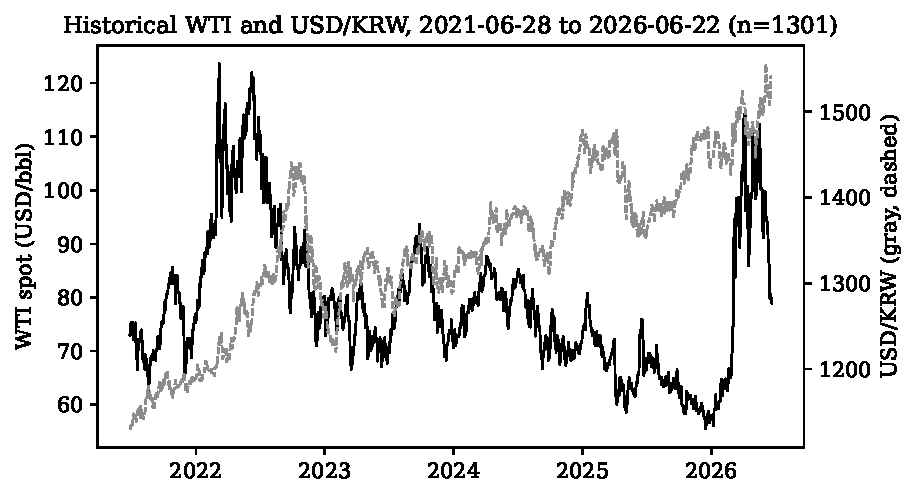
\includegraphics[width=0.75\textwidth]{figures/fig_historical_timeseries.pdf}
\caption{Historical WTI spot and USD/KRW, the calibration source series (Section~\ref{sec:calibration}).}
\label{fig:hist}
\end{figure}

The structural difficulty is this: the KO feature destroys the applicability of the textbook closed-form models (Black-76 for the European vanilla proxy, Turnbull---Wakeman for the Asian-averaging proxy) that a practitioner would otherwise reach for first, because neither model has a barrier term in its analytic derivation. A Longstaff---Schwartz least-squares Monte Carlo (LSMC) regression, by contrast, prices and differentiates the option \emph{on the same simulated paths that determine the KO event}, so the barrier is handled within the same numerical machinery that produces the hedge ratio. This paper's central empirical exercise is to quantify, on an identical common-random-number path bank so that all three delta-estimation methods see the same realized KO/no-KO outcome, how much hedging performance is lost by using a closed-form proxy delta on a barrier structure the proxy model cannot represent.

The remainder of the paper is organized as follows. Section~\ref{sec:litreview} places the model in the existing literature. Section~\ref{sec:dynamics} derives the correlated jump-diffusion dynamics, the quanto double-barrier payoff, and the orthogonal Girsanov transform used to move between the physical measure $\mathbb{P}$ and the pricing measure $\mathbb{Q}$. Section~\ref{sec:calibration} documents the calibration of the WTI jump/diffusion parameters from historical data and the variance-decomposition hazard this creates. Section~\ref{sec:numerical} gives the full numerical formulation: the Longstaff---Schwartz backward-induction algorithm, the corrected 5-term regression basis, the closed-form regression delta, and the log-space Brownian bridge barrier correction. Section~\ref{sec:results} reports the empirical baseline results. Section~\ref{sec:sensitivity} reports sensitivity studies. Section~\ref{sec:pqval} validates the model and the numerical scheme together: the P/Q measure separation directly against simulation, then the scheme's approximation layers removed entirely via a jump-adapted exact simulation at 200{,}000 paths, with measured error decomposition, convergence, a dual price bound, and an Esscher-consistent risk-premium tilt. Section~\ref{sec:discussion} discusses the central technical tension the results expose. Section~\ref{sec:limitations} catalogs the model's limitations, and Section~\ref{sec:conclusion} concludes.

\section{Literature Review}
\label{sec:litreview}

The theoretical foundation for the jump-diffusion dynamics used throughout is Merton (1976), who first formalized a diffusion process punctuated by a compound Poisson jump component and showed that, because jump risk cannot be spanned by continuously-traded instruments, the resulting market is incomplete. Longstaff and Schwartz (2001) supply the numerical engine: least-squares regression of the discounted continuation value onto a low-order polynomial basis of the state variables, evaluated only on in-the-money paths, which turns the pricing of an American-style (or any early-exercise or path-dependent) claim into a tractable backward-induction regression problem. This paper's American engine is a direct, KO-barrier-augmented application of that method; its Asian engine likewise migrates to the same LSMC regression machinery specifically because the KO barrier cannot be represented in a closed-form Asian pricing model.

Two closed-form benchmarks are used explicitly as proxies against which the regression delta is compared. Black (1976) supplies the forward-based closed-form option price used for the European vanilla proxy leg; Turnbull and Wakeman (1991) supply the moment-matching closed-form approximation for the arithmetic-average Asian proxy leg. Neither model has any mechanism to represent a discrete monitored barrier, which is precisely the property this paper exploits: both are deliberately used \emph{as if} they were adequate for a KO structure, so that the resulting hedging degradation can be measured and not merely asserted. Finally, Garman and Kohlhagen (1983) supplies the closed-form FX option formula used wherever a standalone currency option valuation is required in the surrounding sensitivity and diagnostic machinery (in particular the FX leg's own delta terms feeding the one-for-one coupling $\delta_{FX}=\delta_{WTI}$ that the reference point $c=1$ imposes). The correlation coupling between the two legs is priced here as Reiner (1992) characterizes it, as a genuine quanto drift adjustment, but recovered by joint correlated simulation and not by applying his closed-form adjustment directly, for a simple reason: no closed form of that kind survives the addition of a discretely monitored double barrier.

The discrete-monitoring barrier correction used throughout (Section~\ref{sec:bridge}) is not derived from first principles here; it is the continuity correction of Broadie, Glasserman, and Kou (1997), who show that a barrier monitored at $n$ discrete dates can be priced, to a good approximation, by shifting the barrier by $\pm\beta\sigma\sqrt{\Delta t}$ and applying the continuous-monitoring formula, or, as implemented in this paper's regression engine, by a direct Brownian-bridge touch-probability test on each discretization interval. The contribution here is the correction's integration into an LSMC regression pipeline for a two-asset quanto structure, and the direct measurement, in Section~\ref{sec:ejumpmeasured}, of the residual gap the correction leaves against jump risk it was not designed to see.

The jump-diffusion literature's central structural consequence, market incompleteness under discontinuous trajectories, is the reason a diversifiable jump-risk premium survives the $\mathbb{P}\to\mathbb{Q}$ transition in the pricing measure used here (Section~\ref{sec:girsanov}), consistent with the incomplete-markets treatment of jump-diffusion hedging in Cont and Tankov (2004). It is also the direct cause of the finite-difference/regression-delta divergence documented empirically in Section~\ref{sec:fdcheck}: Broadie and Glasserman (1996) establish, for simulation-based Greeks generally, that pathwise and finite-difference estimators can diverge sharply for payoffs with discontinuities of this kind, and a regression fitted on a polynomial basis over a finite, discretely-jumping path set inherits the same structural difficulty and not escaping it. Section~\ref{sec:fdcheck} accordingly measures the magnitude of this known phenomenon on the specific barrier-quanto structure studied here.

What none of these strands directly supplies is a covariance-aware hedge ratio for two legs coupled through a shared barrier and a shared jump component, and not through a simple linear correlation in continuous-time diffusion alone. The cross-hedging tradition of Anderson and Danthine (1981) and its currency extension in Adler and Dumas (1984) optimizes \emph{static} hedge ratios for futures positions, a single number chosen once, and has no object corresponding to a delta recomputed daily on an option whose barrier can extinguish it; its optimality conditions do not speak to a coupling rule applied at every rebalancing date. The unconstrained, single-period version of that same optimization is the minimum-variance hedge ratio of Ederington (1979), and the closed-form multiplier $c^\star$ of Section~\ref{sec:cstar} is this classical estimator, re-derived from the affine per-path cost decomposition of this specific, path-dependent, jump-diffusion structure and not from a new estimation principle. What is new is the structure-specific derivation of that formula, together with the finding that the natural reference point $c=1$ (full pass-through, the setting an independent per-asset treatment defaults to) sits on the expensive, worsening arm of the variance parabola it defines. The quanto literature, from Reiner's drift-adjustment result onward, is a \emph{valuation} literature: it prices the correlation coupling but leaves open the hedging problem that coupling implies, in which two correlated legs carry two notionals and one must be sized against the other. And the barrier-option hedging literature, including the continuity-correction result of Broadie, Glasserman, and Kou (1997), concentrates on the single-underlying discontinuity at the barrier, the delta's explosion near the knock-out level, and not on cross-asset notional sizing. None of these strands examines a covariance-aware hedge ratio for a structure coupled through a shared barrier and a shared jump component. Deriving one in closed form, and measuring what an independent, per-asset treatment costs relative to it, is this paper's contribution.

\section{Asset Dynamics and P/Q Separation}
\label{sec:dynamics}

\subsection{Two-Asset Correlated Jump-Diffusion SDE}
\label{sec:sde}

Let $S_1(t)$ denote the WTI crude price and $S_2(t)$ the USD/KRW exchange rate, both evolving under the physical measure $\mathbb{P}$. $S_1$ is modeled as a jump-diffusion process to capture the empirically fat-tailed, discontinuous behavior of energy prices; $S_2$ is modeled as a standard correlated geometric Brownian motion:
\begin{align}
\frac{dS_1(t)}{S_1(t^-)} &= (\mu_1^{\mathbb P}-\lambda\kappa)\,dt + \sigma_1\,dW_1(t) + d\!\left(\sum_{j=1}^{N(t)}(e^{Y_j}-1)\right) \\
\frac{dS_2(t)}{S_2(t)} &= \mu_2^{\mathbb P}\,dt + \sigma_2\,dW_2(t) \\
dW_1(t)\cdot dW_2(t) &= \rho\,dt \\
\kappa &= \mathbb E[e^{Y}-1] = \exp\!\left(\theta_J+\tfrac12\delta_J^2\right)-1
\end{align}
$N(t)$ is a Poisson counting process with intensity $\lambda$, independent of $W_1,W_2$; each jump multiplies the pre-jump price by $e^{Y_j}$, with the log-jump-size $Y_j$ drawn i.i.d.\ from a normal distribution,
\begin{align}
Y_j \sim \mathcal N(\theta_J,\delta_J^2).
\end{align}

For simulation, the SDE of Section~\ref{sec:sde} is discretized on a uniform grid $t_i=i\Delta t$, $i=0,\ldots,n$, $\Delta t = T/n$, using an Euler---Maruyama scheme with the compound Poisson jump superimposed once per step. On the risk-neutral measure $\mathbb Q$ constructed in Section~\ref{sec:girsanov} (drift $\mu_1^{\mathbb P}\to r_{US}$, $\mu_2^{\mathbb P}\to r_{KRW}-r_{US}$), the one-step update is
\begin{align}
\varepsilon_1 &\sim \mathcal N(0,1), \qquad \varepsilon_2^{\perp} \sim \mathcal N(0,1), \qquad \varepsilon_2 = \rho\varepsilon_1 + \sqrt{1-\rho^2}\,\varepsilon_2^{\perp} \\
N_i &\sim \mathrm{Poisson}(\lambda\Delta t), \qquad J_i = \sum_{j=1}^{N_i} Y_j, \qquad Y_j \overset{\text{iid}}{\sim} \mathcal N(\theta_J,\delta_J^2) \\
S_1(t_{i+1}) &= S_1(t_i)\,\exp\!\left[\left(r_{US}-\lambda\kappa-\tfrac12\sigma_1^2\right)\Delta t + \sigma_1\sqrt{\Delta t}\,\varepsilon_1 + J_i\right] \\
S_2(t_{i+1}) &= S_2(t_i)\,\exp\!\left[\left(r_{KRW}-r_{US}-\tfrac12\sigma_2^2\right)\Delta t + \sigma_2\sqrt{\Delta t}\,\varepsilon_2\right]
\end{align}
The number of jumps $N_i$ within a single step is itself simulated (not merely a 0/1 indicator), so that more than one jump landing in the same daily interval is representable, and the aggregate jump contribution $J_i$ is the sum of that many independent draws of $Y_j$. The shared standard normal $\varepsilon_1$ drives both the diffusive part of $S_1$ and, through the $\rho\varepsilon_1$ term, the correlated part of $S_2$'s shock $\varepsilon_2$; this is the same Cholesky-style construction formalized in Section~\ref{sec:girsanov}.

The introduction of the Poisson jump component converts the asset manifold from complete to incomplete. In a pure diffusion setting, the Black-Scholes replication argument holds exactly: a continuously-rebalanced portfolio of the underlying and a risk-free bond spans every contingent claim, because the only source of risk is a continuous Brownian increment that a continuously-adjusted delta position can offset instantaneously. A Poisson jump differs from a diffusive move in kind as well as in size: it is an instantaneous, discontinuous repricing that occurs at an unpredictable stopping time, and no finite adjustment made an instant before the jump can offset a discontinuity whose magnitude is drawn from a continuous distribution \emph{after} the jump has already occurred. Because the space of possible jump outcomes cannot be spanned by a finite number of continuously-traded hedging instruments, the market admits infinitely many equivalent martingale measures and not the single one guaranteed under diffusion-only market completeness, and the choice among them is governed by the market's aggregate risk aversion toward jump risk specifically, a diversifiable-risk assumption this paper follows explicitly (Section~\ref{sec:girsanov}) in choosing $\lambda,\theta_J,\delta_J$ to be measure-invariant.

The compensator term $-\lambda\kappa\,dt$ embedded in the drift is not an optional convention; it is required to keep the model's own stated drift parameter, $\mu_1^{\mathbb P}$, meaning what it is defined to mean. The compound Poisson jump term $\sum_{j=1}^{N(t)}(e^{Y_j}-1)$ has, by construction, an instantaneous expected contribution of $\lambda\,\mathbb E[e^Y-1]\,dt=\lambda\kappa\,dt$ to the process. If this expected jump contribution were left inside the total drift without being netted out, the realized expected growth rate of $S_1$ would exceed $\mu_1^{\mathbb P}$ by exactly $\lambda\kappa$, silently double-counting the jump component's mean inside a parameter that is supposed to represent the asset's total observed physical-measure drift. Subtracting $\lambda\kappa\,dt$ from the diffusive drift restores $\mu_1^{\mathbb P}$ as the asset's true expected growth rate under $\mathbb P$, and under the risk-neutral measure this same compensator structure (with $\mu_1^{\mathbb P}$ replaced by $r_{US}$) is the algebraic condition that keeps the discounted price process a local martingale, i.e. the condition without which no self-consistent pricing measure exists at all.

\subsection{Quanto Double-Knock-Out Payoff Construction}
\label{sec:payoff}

Before turning to measure separation and calibration, it is worth writing the contract this paper prices and hedges out in full, since every subsequent formula is a derivative of this single object. The importer's exposure is to a monthly barrel requirement whose dollar cost, once converted to KRW, depends multiplicatively on both $S_1$ and $S_2$; the structure is built to offset that multiplicative joint exposure, at the smaller premium a barrier affords, by paying the same product $S_1 \cdot S_2$ only above a strike and only while WTI has stayed within a monitored corridor. Writing $K$ for the strike, $U$ and $L$ for the upper and lower KO barriers ($U=120$, $L=50$ USD/bbl in the production configuration), and $\tau_{KO}=\inf\{t : S_1(t)\ge U \text{ or } S_1(t)\le L\}$ for the first barrier-hitting time, the three payoff variants studied in this paper are:
\begin{align}
V^{\text{Eur}}(T) &= \mathrm{barrels}\cdot \max(S_1(T)-K,0)\cdot S_2(T)\cdot\mathbf 1\{\tau_{KO}>T\} \\
V^{\text{Amer}}(\tau) &= \sup_{\tau\,\le\, T\wedge\tau_{KO}}\ \mathbb E^{\mathbb Q}\!\left[e^{-r_{US}\tau}\,\mathrm{barrels}\cdot\max(S_1(\tau)-K,0)\cdot S_2(\tau)\ \middle|\ \mathcal F_0\right] \\
V^{\text{Asian}}(T) &= \mathrm{barrels}\cdot \max\!\big(\bar S_1(T)-K,0\big)\cdot S_2(T)\cdot\mathbf 1\{\tau_{KO}>T\}, \qquad \bar S_1(T) = \frac{1}{m}\sum_{k=1}^{m} S_1(t_k)
\end{align}
where the supremum in the American payoff ranges over $\mathbb Q$-measure stopping times $\tau$ that are themselves bounded by the first KO time $\tau_{KO}$ (once the barrier is hit the contract is dead and no exercise decision remains to be made), and $\bar S_1(T)$ in the Asian payoff is the arithmetic average of WTI over the $m$ pre-specified averaging dates $t_1<\cdots<t_m\le T$.

Each of these payoffs multiplies a WTI-leg quantity by the \emph{floating} terminal FX rate $S_2(T)$ and not by a rate fixed at inception; this is the source of the "quanto" correlation coupling referenced throughout the paper. Because $S_1(T)$ and $S_2(T)$ are jointly, non-trivially correlated under the model of Section~\ref{sec:sde} (through the shared shock $\rho\varepsilon_1$ appearing in both legs' discretized increments), the risk-neutral expectation of the product does not factor into a product of expectations:
\begin{align}
\mathbb E^{\mathbb Q}\!\big[\max(S_1(T)-K,0)\cdot S_2(T)\big] \;\ne\; \mathbb E^{\mathbb Q}\!\big[\max(S_1(T)-K,0)\big]\cdot \mathbb E^{\mathbb Q}\!\big[S_2(T)\big].
\label{eq:quantocouple}
\end{align}
The inequality in \eqref{eq:quantocouple} is correct as stated, and it is tempting to read it as saying that $\rho$ enters the price. It does not. The payoff converts at the \emph{realized} terminal rate rather than at a rate fixed in advance, and that is precisely the case in which a change of numeraire removes the correlation entirely.

\begin{proposition}[Factorization]
\label{prop:factor}
Let $N(t)=S_2(t)e^{r_{US}t}$ be the KRW value of the USD money-market account, a traded KRW asset, and let $\mathbb Q^{US}$ be the measure it induces. For any payoff of the form $X(T)\cdot S_2(T)$ with $X$ measurable with respect to the $S_1$ path,
\begin{equation}
V(0)\;=\;\mathbb E^{\mathbb Q^{KRW}}\!\big[e^{-r_{KRW}T}X(T)S_2(T)\big]\;=\;S_2(0)\,e^{-r_{US}T}\,\mathbb E^{\mathbb Q^{US}}\!\big[X(T)\big],
\label{eq:factorization}
\end{equation}
in which neither $\rho$ nor $\sigma_2$ appears.
\end{proposition}

\noindent The proof is the numeraire change itself: $V(0)=N(0)\,\mathbb E^{\mathbb Q^{US}}[X(T)S_2(T)/N(T)] = S_2(0)e^{-r_{US}T}\mathbb E^{\mathbb Q^{US}}[X(T)]$. Setting $X(T)=\max(S_1(T)-K,0)\mathbf 1\{\text{no barrier touch}\}$ gives this paper's structure. The correlation adjustment $-\rho\sigma_1\sigma_2$ that a KRW-numeraire treatment applies to the drift of $S_1$ is exactly offset by the $+\rho\sigma_1\sigma_2$ generated by the covariance between $X(T)$ and $S_2(T)$; the two cancel, which is what \eqref{eq:factorization} records. Direct simulation confirms it, and confirms it with the barrier in place rather than only for the vanilla case: repricing the double-knock-out payoff at $\rho\in\{-0.5,\,0,\,0.0876,\,0.5\}$ under the correctly-specified measure moves the value by at most $0.6\%$, non-monotonically in $\rho$ and so within Monte Carlo error, against a factorized closed form agreeing to the same tolerance. The survival probability is likewise flat across $\rho$ ($0.741$--$0.743$). This is what \eqref{eq:factorization} predicts: the numeraire change shifts the drift of $S_1$ from $r_{US}-\rho\sigma_1\sigma_2$ under $\mathbb Q^{KRW}$ to $r_{US}$ under $\mathbb Q^{US}$, so the first-passage law that governs the barrier is itself $\rho$-free.

This is a structural fact about the instrument and not a defect in it, but it has three consequences the rest of the paper depends on. First, the label ``quanto'' is used here in its loose desk sense, for a two-asset structure whose payoff is denominated across currencies, and not in the technical sense of a fixed-conversion-rate contract carrying a correlation-dependent drift adjustment: this structure carries no such adjustment. A genuine quanto would convert at a rate fixed at inception, and only then would $\rho$ survive into the price. Second, Proposition~\ref{prop:factor} \emph{is} the homogeneity result that Section~\ref{sec:structdelta} derives independently and uses to obtain $\delta_{FX}=V/S_2$; the FX-delta results of this paper are therefore consequences of the factorization rather than of any correlation coupling, and they are strengthened by it, since \eqref{eq:factorization} makes the structure's entire FX exposure its own carrying value by construction. Third, the correlation between the two legs remains economically real on the \emph{hedging} side, where it drives the covariance $\mathrm{Cov}(A,B)$ that determines $c^\star$ in Section~\ref{sec:cstar}; it is the pricing channel, not the hedging channel, that the factorization closes.

All three benchmark engines draw their FX multiplication from the same jointly-simulated bank, so the FX leg is never a source of divergence between them (Section~\ref{sec:baseline}); only the barrier treatment is.

\subsection{Orthogonal Girsanov Transform and Risk Premium Isolation}
\label{sec:girsanov}

Write the correlated shocks in an orthogonal basis, $\epsilon_1=z_1$, $\epsilon_2=\rho z_1+\sqrt{1-\rho^2}\,z_2$, with market prices of risk $\theta_1=(\mu_1^{\mathbb P}-r_{US})/\sigma_1$ and $\theta_2=(\mu_2^{\mathbb P}-(r_{KRW}-r_{US}))/\sigma_2$. Shifting $\epsilon_2$ by $\theta_2$ directly would price the WTI risk premium twice, since $\epsilon_2$ already carries a $\rho$-weighted share of the $z_1$ shock that $\theta_1$ shifts; the orthogonalized currency premium, acting purely on $z_2$, is
\begin{align}
\theta_{2,\text{indep}} = \frac{\theta_2 - \rho\,\theta_1}{\sqrt{1-\rho^2}},
\end{align}
and with the Girsanov density built from $(\theta_1$ on $z_1$, $\theta_{2,\text{indep}}$ on $z_2)$ the $\mathbb Q$-drifts reduce exactly to $r_{US}$ and $r_{KRW}-r_{US}$ with no correlation leakage. Section~\ref{sec:pqval} validates the construction twice: exactly, against closed-form drift moments; and inexactly, by likelihood-ratio reweighting of the path-dependent KO payoff, whose residual localizes numerical and not theoretical error.

\section{Calibration of WTI Jump/Diffusion Inputs}
\label{sec:calibration}

A naive historical volatility estimator measures the \emph{total} quadratic variation, diffusion plus jumps. Assigning it entirely to $\sigma_1$ and then layering Poisson jumps on top simulates strictly more variance than was ever observed, silently inflating both the premium and every downstream hedge cost. The calibration must therefore \emph{split} the observed variance and not duplicate it.

\subsection{Asymmetric Up/Down EM Decomposition}
\label{sec:emcalib}

The production calibration resolves this by a truncated Poisson-mixture EM decomposition of the historical WTI log-return series, estimating an \emph{up}-jump and a \emph{down}-jump regime separately, since energy-price shocks are empirically asymmetric, with downside dislocations sharper than upside recoveries. Each daily return is treated as a mixture over six components (no jump; one or two jumps of either sign; one of each), the E-step assigning posterior memberships against Gaussian densities that all include the diffusive variance $\sigma_1^2\Delta t$, and the M-step re-estimating $(\lambda,\theta_J,\delta_J)$ per regime and $\sigma_1$ from the no-jump component, iterated to log-likelihood convergence; the full mixture construction is given in Appendix~\ref{app:em}.

Because every downstream engine in this paper (Sections~\ref{sec:sde}---\ref{sec:numerical}) simulates a single symmetric jump distribution and not two asymmetric regimes, the fitted $(\lambda_{up},\theta_{J,up},\delta_{J,up})$ and $(\lambda_{dn},\theta_{J,dn},\delta_{J,dn})$ pairs are moment-matched to a single equivalent Poisson-normal jump $(\lambda,\theta_J,\delta_J)$ by matching total jump intensity, the aggregate first moment, and the aggregate second moment of the jump-size distribution:
\begin{align}
\lambda &= \lambda_{up}+\lambda_{dn} \\
\theta_J &= \frac{\lambda_{up}\,\theta_{J,up} + \lambda_{dn}\,\theta_{J,dn}}{\lambda} \\
\delta_J^2 &= \frac{\lambda_{up}\big(\theta_{J,up}^2+\delta_{J,up}^2\big) + \lambda_{dn}\big(\theta_{J,dn}^2+\delta_{J,dn}^2\big)}{\lambda} \;-\; \theta_J^2
\end{align}
The three lines match, in order, the total arrival rate, the intensity-weighted mean (preserving the compensator $\lambda\kappa$ of Section~\ref{sec:sde}), and the pooled second moment, an exact two-to-one variance decomposition.

Table~\ref{tab:asymjump} reports the fitted regimes directly, and not only the symmetrized pair the downstream engines consume. Down-jumps arrive nearly twice as often as up-jumps ($\lambda_{dn}=4.462$ vs.\ $\lambda_{up}=2.328$ per year), are roughly $9\%$ larger in magnitude ($|\theta_{J,dn}|=8.75\%$ vs.\ $\theta_{J,up}=8.04\%$), and are 66\% more volatile ($\delta_{J,dn}=2.78\%$ vs.\ $\delta_{J,up}=1.68\%$). The asymmetry is a measured property of the return history ($n_{up}=12$, $n_{dn}=23$ classified jump days).

A note on what this estimator is, because the paper's earlier drafts described it loosely. Jump days are identified by a $k$-sigma threshold rule and the intensity is their annualised count: $35\times252/1300=6.7846$ per year reproduces the figure the engines use to seven digits, and the two regime intensities are $12\times252/1300$ and $23\times252/1300$. It is a threshold classifier followed by moment-matching within each regime, not the likelihood-maximising mixture that ``EM'' would imply, and the symmetrized triple $(\lambda,\theta_J,\delta_J)=(6.7846,-0.0299,0.08443)$ is what every engine in this paper consumes. Re-deriving the symmetrization from the rounded regime values displayed above returns $\delta_J=0.0834$ rather than $0.08443$, a $1.2\%$ difference that is an artifact of the rounding rather than a second estimate. The estimation sample is the 1{,}300 paired returns of the price history; the figure of 1{,}299 quoted elsewhere in this paper and its companion differs by one observation and moves $\sigma_1$, $\sigma_2$ and $\rho$ in the fifth decimal place.

\begin{table}[h]
\centering
\small
\begin{tabular}{lrrrr}
\toprule
Regime & $\lambda$ (jumps/yr) & $\theta_J$ & $\delta_J$ & $n$ days \\
\midrule
Up-jump ($r>0$)   & 2.328 & $+8.04\%$ & $1.68\%$ & 12 \\
Down-jump ($r<0$) & 4.462 & $-8.75\%$ & $2.78\%$ & 23 \\
\midrule
Symmetrized (as used by the engines) & 6.7846 & $-2.99\%$ & $8.443\%$ & 35 \\
\bottomrule
\end{tabular}
\caption{Fitted up/down jump regimes and their moment-matched symmetrization, from the 1,299-day WTI daily log-return history (k=3 robust threshold).}
\label{tab:asymjump}
\end{table}

The resulting decomposition: total historical WTI volatility $\sigma_1=0.3946$ splits into a diffusive $\sigma_1 = 0.3242$ and a symmetrized jump component $(\lambda,\theta_J,\delta_J)=(6.7846,\,-0.0299,\,0.08443)$. The negative mean jump size is the asymmetric fit's quantitative trace surviving symmetrization: the larger, more frequent down-jump regime pulls $\theta_J$ negative under intensity weighting. The FX leg calibrates to $\sigma_2 = 0.0926$ with WTI---FX correlation $\rho = 0.0876$, the quantity the orthogonal Girsanov construction of Section~\ref{sec:girsanov} isolates. Whether the up/down asymmetry itself matters for barrier risk is testable: simulating the genuine two-regime process against the symmetrized draw on matched seeds moves barrier-touch probabilities by under $0.1$ percentage points even from starting points near the barrier, because the $32.4\%$ diffusive volatility dominates touch dynamics over sub-annual horizons, so the symmetrization is quantitatively adequate for this structure and not merely tractable.

\section{Numerical Model Formulation}
\label{sec:numerical}

\subsection{Path Simulation and the Longstaff---Schwartz Backward-Induction Algorithm}
\label{sec:lsmcalgo}

Pricing and hedging every structure in this paper reduces, algorithmically, to a single backward-induction procedure applied to a bank of $N$ jointly-simulated $(S_1,S_2)$ paths built from the discretization of Section~\ref{sec:sde}. Writing $\hat V_p(t_i)$ for the estimated value of the contract on path $p$ at step $i$, the procedure is:

\begin{enumerate}
\item \textbf{Forward simulation.} Simulate all $N$ paths forward from $t_0$ to $t_n=T$ using the one-step update of Section~\ref{sec:sde}, recording $S_1(t_i,p)$, $S_2(t_i,p)$ at every step, and separately recording the first barrier-hitting step $i_{KO}(p)$ (identified via the Brownian-bridge test of Section~\ref{sec:bridge}, applied between each pair of consecutive recorded steps).
\item \textbf{Terminal initialization.} At $i=n$, set $\hat V_p(t_n) = \max(S_1(t_n,p)-K,0)\cdot S_2(t_n,p)$ for the European and American payoffs (Section~\ref{sec:payoff}), or the corresponding running-average intrinsic value $\max(\bar S_1(T,p)-K,0)\cdot S_2(t_n,p)$ for the Asian payoff, on every path not already knocked out by $i_{KO}(p)\le n$; knocked-out paths carry a value of zero from their KO step onward.
\item \textbf{Backward loop.} For $i=n-1,n-2,\ldots,1$:
  \begin{enumerate}
  \item Identify the in-the-money (ITM) path subset $\mathcal I_i = \{p : S_1(t_i,p) > K \text{ and } i < i_{KO}(p)\}$.
  \item On $\mathcal I_i$ only, regress the one-step-discounted continuation value $e^{-r_{US}\Delta t}\hat V_p(t_{i+1})$ against the 5-term polynomial basis of Section~\ref{sec:basis} evaluated at $(v_1,v_2)$ at $t_i$, by ordinary least squares, to obtain the fitted coefficients $\beta_0(t_i),\ldots,\beta_5(t_i)$.
  \item For American paths only: on $\mathcal I_i$, compare the fitted continuation value $\tilde C(S_1(t_i,p),S_2(t_i,p))$ against the immediate exercise value $\max(S_1(t_i,p)-K,0)\cdot S_2(t_i,p)$; where exercise value exceeds continuation value, overwrite $\hat V_p(t_i)$ with the exercise value and mark path $p$ as exercised at $t_i$ (removing it from all subsequent backward steps).
  \item On every path not exercised at this step, set $\hat V_p(t_i) = e^{-r_{US}\Delta t}\hat V_p(t_{i+1})$ (out-of-the-money and previously-alive paths simply carry the discounted future value backward unchanged; the regression is used only to make the exercise decision, never to replace the realized future cash flow, which is the defining feature of the Longstaff---Schwartz estimator relative to a naive plug-in of the fitted surface).
  \end{enumerate}
\item \textbf{Price and Greeks.} The step-0 price is $\hat V(t_0) = \frac{1}{N}\sum_{p=1}^N \hat V_p(t_0)$ (the cross-sectional average of the backward-propagated cash flows), and the fitted coefficient set $\{\beta_0(t_i),\ldots,\beta_5(t_i)\}_{i=1}^{n}$ retained from step 3(b) at every time step is what Section~\ref{sec:delta} differentiates analytically to obtain the hedging delta at each rebalancing date, so no separate pricing pass is required to extract the Greek once the backward loop above has been run once.
\end{enumerate}

This is the standard Longstaff---Schwartz (2001) least-squares Monte Carlo estimator, with two structure-specific modifications relative to its textbook presentation: the ITM path subset in step 3(a) additionally excludes any path already knocked out ($i<i_{KO}(p)$), so the regression is never fitted using post-barrier paths whose future cash flow is trivially zero; and step 3(c) (the exercise comparison) is applied only for the American engine, so that the identical steps 1, 2, 3(a), 3(b), 3(d), and 4, unmodified, also constitute the full pricing and delta-extraction procedure for the barrier-only European and Asian engines, with early exercise simply never triggering.

\subsection{Corrected State-Variable Normalization and the 5-Term Polynomial Basis}
\label{sec:basis}

The cross-sectional LSMC regression at each time step fits the discounted continuation value against a 5-term polynomial in two normalized state variables (five regressor terms plus a constant, six coefficients $\beta_0,\ldots,\beta_5$ in total, the count referenced throughout this paper as ``5-term,'' and, where every coefficient is tallied explicitly as in Table~\ref{tab:basis}, as ``6-term''). Writing $K$ for the option strike (set at-the-money-forward, $K=S_1(0)$, in the production configuration) and $S_2(0)$ for the inception FX spot, the normalized variables are
\begin{align}
v_1 &= \frac{S_1}{K} \\
v_2 &= \frac{S_2}{S_2(0)}
\end{align}
so that $v_1,v_2\approx 1$ near inception and both regressors move in direct, not inverse, proportion to the underlying spot. (An inverted definition $v_1=K/S_1$ would explode as $S_1\to 0$, a numerically valid state in a distressed commodity path, and would destabilize the regression's matrix conditioning; the production code avoids this by construction.) The continuation value surface is then
\begin{align}
\tilde C(S_1,S_2) = \beta_0+\beta_1 v_1+\beta_2 v_2+\beta_3 v_1^2+\beta_4 v_2^2+\beta_5 v_1 v_2
\end{align}
fitted by ordinary least squares, in-the-money paths only, independently at each of the $217$ discrete time steps spanning the $T=0.833$-year (approximately ten-month) horizon. This is step 3(b) of the backward-induction algorithm of Section~\ref{sec:lsmcalgo}, and the six coefficients solved at every step form the full pricing surface that algorithm accumulates. Section~\ref{sec:errdecomp} (Table~\ref{tab:basis}) bounds how much this particular basis choice matters by pricing the same structure under a strictly larger cubic basis, a genuinely non-polynomial exponentially-weighted Laguerre-function basis, and a payoff-kink-augmented basis, bounding the basis effect at one percent, and showing that kink-aware terms are no-ops under ITM-only fitting, since the hinge is linear on the fitted region.

\subsection{The Closed-Form LSMC Regression Delta}
\label{sec:delta}

The hedging gradient is obtained analytically by differentiating the fitted polynomial surface with respect to $S_1$ and rescaling into FX-adjusted notional terms, using $\partial v_1/\partial S_1 = 1/K$:
\begin{align}
\delta_{WTI}^{\text{Amer}} &= \mathrm{clip}_{[0,1]}\!\left(\frac{1}{S_2}\cdot\frac{1}{K}\left(\beta_1+2\beta_3 v_1+\beta_5 v_2\right)\right) \\
\delta_{FX} &= c\cdot\delta_{WTI}, \qquad c=1.0
\end{align}
This is the exact closed-form derivative of the fitted regression surface; no finite-difference re-pricing is required, so the delta is available at zero marginal simulation cost once $\beta_0,\ldots,\beta_5$ are known at a given step. Each term of the polynomial maps to an interpretable hedging quantity: $\beta_1$ is the surface's static linear delta; $2\beta_3 v_1$ is a moneyness-dependent acceleration term acting as an implicit local gamma; $\beta_5 v_2$ injects the cross-asset correlation directly into the WTI hedge ratio, so that a shift in the FX leg alone can move the required WTI hedge notional. The $\mathrm{clip}_{[0,1]}$ bound is an operational constraint on the regression's own fitting noise, which is unbounded in principle and would otherwise occasionally instruct the desk to hold an over-leveraged position. It is not a costless one, and the cost falls on precisely the feature this paper is about. An up-and-out call has a genuinely \emph{negative} delta as spot approaches the upper barrier, because a further rise makes extinction more likely and the option less valuable; that sign reversal is the most characteristic behavior of a barrier delta, and the lower clip at zero removes it. The estimator this paper calls barrier-aware is therefore barrier-aware everywhere except in the region where the barrier matters most, and the comparison against barrier-blind proxies in Section~\ref{sec:hedgecost} is correspondingly conservative: it understates what an unclipped barrier-aware delta would deliver, since the clip damages the regression delta and leaves the proxies, which never produce negative deltas either, untouched. Section~\ref{sec:limitations} records this as an open item; an unclipped re-run, reporting both the hedge-cost change and the frequency with which the raw delta goes negative near the upper barrier, is the natural next measurement and is not performed here. Section~\ref{sec:fdcheck} documents empirically how large the gap between this closed-form regression delta and the numerical finite-difference delta actually is, and where in the option's life that gap is largest.

\subsection{Log-Space Brownian Bridge Barrier Correction: Upper and Lower Barriers}
\label{sec:bridge}

A discretely-recorded path can cross a barrier between two observations and revert, leaving no trace on the grid, a systematic \emph{under}-detection that would overprice the structure. This is the discrete-monitoring bias formalized by Broadie, Glasserman, and Kou (1997); the correction implemented here is their bridge-probability treatment applied directly on each discretization interval, and not their alternative barrier-shift approximation, since the per-step conditional touch probability is available in closed form once the interval's endpoints are known. The correction applies, on each step with both recorded endpoints interior to $[L,U]$, the exact Brownian-bridge touch probability in log-space for each barrier:
\begin{align}
p_{up} &= \exp\!\left(\frac{-2\ln(U/S_1^{\text{prev}})\,\ln(U/S_1)}{\sigma_1^2\,\Delta t}\right), \qquad
p_{dn} = \exp\!\left(\frac{-2\ln(S_1^{\text{prev}}/L)\,\ln(S_1/L)}{\sigma_1^2\,\Delta t}\right),
\end{align}
each compared against an independent uniform draw once per step; endpoints on or beyond a barrier are direct discrete touches. A positive bridge test updates only the KO flag and index $i_{KO}(p)$, never the recorded values.

Both $p_{up}$ and $p_{dn}$ are mathematically exact under the strict assumption that the path between the two endpoints is continuous. Under the model of Section~\ref{sec:sde}, that assumption is only approximately true: a genuine Poisson jump can teleport the price across a barrier discontinuously, a scenario the continuous bridge formula was never derived to capture, since it has no mechanism for a jump that occurs \emph{between} the two conditioning endpoints and is not itself one of the two recorded values. Formally, the true step-conditional touch probability decomposes as
\begin{equation}
\label{eq:jumpgap}
\mathbb P\big(\tau_{KO}\in(t_i,t_{i+1}]\ \big|\ S_1(t_i),S_1(t_{i+1})\big) \;=\; p_{up} \;+\; \mathcal E_{\mathrm{jump}}(\lambda,\theta_J,\delta_J;\Delta t),
\end{equation}
where $\mathcal E_{\mathrm{jump}}\ge0$ collects the paths the bridge test cannot see: a jump lands strictly inside $(t_i,t_{i+1})$, crosses $U$ (or $L$), and reverts in log-price to the interior of $[L,U]$ by $t_{i+1}$, indistinguishable from the two recorded endpoints alone from a jump-free path that stayed inside the barrier throughout. Such a path requires both a jump landing in an interval of length $\Delta t$ (probability $O(\lambda\Delta t)$) \emph{and} that jump crossing a barrier several diffusive standard deviations from the endpoint, so $\mathcal E_{\mathrm{jump}}=O(\Delta t)$ and $\mathcal E_{\mathrm{jump}}\to0$ as $\Delta t\to0$, vanishing at the same order as the Euler---Maruyama discretization error the bridge correction was already built to control. Given the daily granularity of the production grid (217 steps over 0.833 years, i.e.\ roughly one step per trading day), this residual is small in expectation, since a typical single jump of magnitude $\theta_J\pm\delta_J\approx-3.0\%\pm8.4\%$ against barriers set at $+52\%/-37\%$ from spot is very unlikely to itself be the difference between touching and not touching the barrier within a single day, and \eqref{eq:jumpgap} makes explicit that it is nonzero.

\section{Empirical Results}
\label{sec:results}

\subsection{Baseline Pricing and the Knock-Out Rate}
\label{sec:baseline}

At the production baseline ($S_1(0)=78.94$ USD/bbl, $S_2(0)=1{,}540.64$ KRW/USD, $r_{US}=4.0\%$, $r_{KRW}=3.5\%$, KO barriers at $50/120$ USD/bbl), the LSMC-priced base premium is KRW $17{,}132.47$ per quanto unit, scaling to a total structure premium of KRW $34{,}264{,}941{,}589$ across the full 2{,}000-contract (2{,}000{,}000 barrel) position. A Shapley-style attribution of this premium across the two legs assigns KRW $15{,}093.75$ (88.1\%) to the WTI leg and KRW $2{,}038.72$ (11.9\%) to the FX leg, consistent with the WTI leg carrying the dominant share of both notional and volatility in this structure.

All hedge simulation results reported below are computed on $n=10{,}000$ independent common-random-number paths, rebalanced daily over 217 steps.

\textbf{The KO rate is not a single invariant number, and reporting it as one number obscures a genuine structural feature of the American engine.} On the shared path bank, the two engines whose stopping rule tests the barrier alone (European with the Black-76 proxy delta, and Asian with the Turnbull---Wakeman proxy delta) report an identical KO rate of $0.4369$, confirming that both engines are evaluated on the same underlying barrier-touch process. The American engine reports a strictly smaller KO rate of $0.2309$, alongside an early-exercise rate of $0.4474$. This is not evidence of a different barrier process for American; it is the direct consequence of early exercise being a competing first-stopping-time event: on any path where the American holder's optimal-stopping rule triggers exercise before the barrier is touched, that path is tallied as "exercised," not "knocked out," even though the identical underlying path, had it been held without an exercise option, would eventually register a barrier touch and would be counted in the 0.4369 figure. The three rates partition the American path population into exercise ($44.74\%$), KO ($23.09\%$), and alive-to-maturity ($32.17\%$), and the correct empirical statement is that the raw barrier-touch frequency on this path bank is $0.4369$, with American's early-exercise feature pre-empting roughly half of what would otherwise have been KO outcomes.

\subsection{Hedge Cost: American LSMC vs. Closed-Form Proxies}
\label{sec:hedgecost}

The primary comparison metric used throughout is \emph{hedge cost}, defined per path as $\mathrm{HC}=\Pi_{\mathrm{option}}-\Pi_{\mathrm{delta}}$, the realized option profit net of total delta-hedge profit. It is distinct from \emph{total P\&L}, which is reported in Tables~\ref{tab:fxsweep} and~\ref{tab:lambdarob} and additionally carries the premium outlay and the physical-leg settlement, so the two are not directly comparable in level; hedge cost which by construction isolates the performance of the delta strategy itself and does not conflate delta quality with the underlying payoff-structure differences between an American, European, and Asian claim. Table \ref{tab:hedgecost} reports the full-population ($n=10{,}000$) mean and standard deviation of hedge cost under each of the three delta-estimation methods.

\begin{table}[h]
\centering
\caption{Hedge cost distribution, full population ($n=10{,}000$), KRW}
\label{tab:hedgecost}
\begin{tabular}{lrr}
\toprule
Engine (delta method) & Mean hedge cost & Std.\ dev.\ hedge cost \\
\midrule
American (LSMC regression) & 4{,}242{,}549{,}693 & 54{,}406{,}045{,}559 \\
European (Black-76 proxy) & 66{,}914{,}895{,}880 & 117{,}398{,}625{,}340 \\
Asian (Turnbull---Wakeman proxy) & 66{,}423{,}885{,}856 & 110{,}073{,}446{,}997 \\
\bottomrule
\end{tabular}
\end{table}

\begin{figure}[h]
\centering
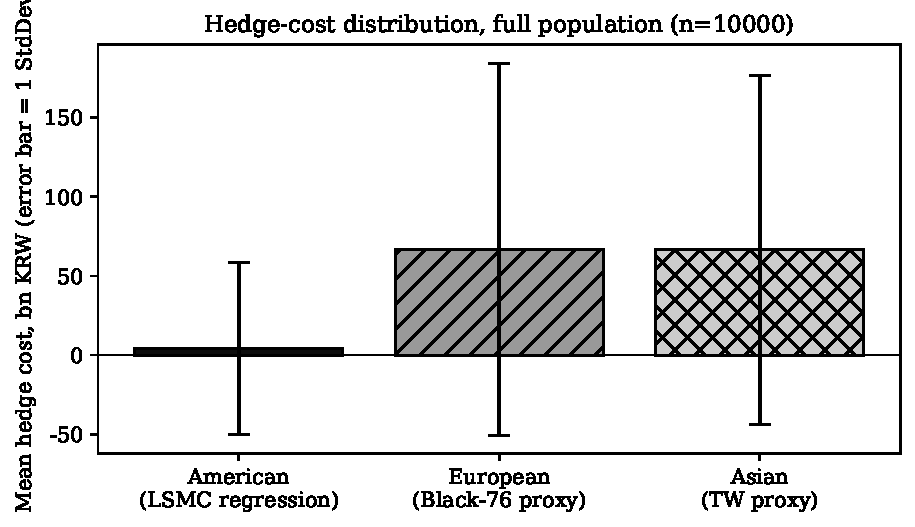
\includegraphics[width=0.72\textwidth]{figures/fig_hedge_cost_distribution.pdf}
\caption{Mean hedge cost and one standard deviation, full population, by delta-estimation method.}
\label{fig:hedgecost}
\end{figure}

The LSMC regression delta's mean hedge cost (KRW 4.24 billion) is smaller than either closed-form proxy's by roughly a factor of fifteen, and its standard deviation is smaller by a factor of two. Because the full-population comparison mixes paths with genuinely different payoff structures (KO'd paths, early-exercised paths, and paths alive to maturity all pool together, and American, European, and Asian pay off differently even conditional on an identical path), a second, cleaner test isolates the $n=3{,}217$ paths ($32.2\%$ of the population) that are simultaneously non-KO and non-early-exercised, the subset on which American and European pay off \emph{identically} ($\max(S_1(T)-K,0)\cdot S_2(T)$ on a shared path), so that any remaining hedge-cost difference is attributable purely to the delta-estimation method and nothing else.

\begin{table}[h]
\centering
\caption{Hedge cost, clean subset (non-KO, non-exercise, $n=3{,}217$), KRW}
\label{tab:hedgecostclean}
\begin{tabular}{lrr}
\toprule
Engine & Mean hedge cost & Std.\ dev.\ hedge cost \\
\midrule
American (LSMC regression) & 26{,}928{,}215{,}657 & 36{,}765{,}911{,}185 \\
European (Black-76 proxy) & 91{,}526{,}694{,}827 & 91{,}558{,}547{,}428 \\
\bottomrule
\end{tabular}
\end{table}

\begin{figure}[h]
\centering
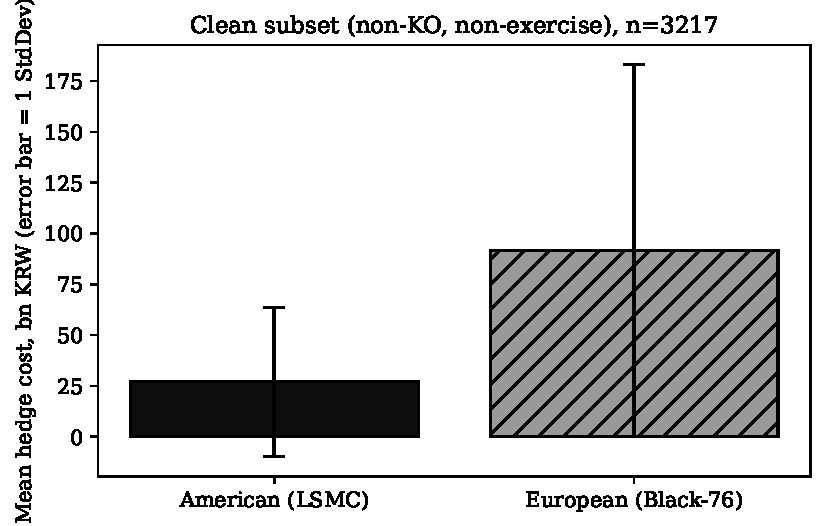
\includegraphics[width=0.62\textwidth]{figures/fig_hedge_cost_clean_subset.pdf}
\caption{Hedge cost, clean (non-KO, non-exercise) subset: pure delta-method comparison.}
\label{fig:cleansubset}
\end{figure}

Even with payoff-structure confounding fully removed, the LSMC regression delta's mean hedge cost is KRW $64.6$ billion lower and its standard deviation is roughly $2.5\times$ smaller than the Black-76 proxy delta's, on paths where both models are pricing and differentiating literally the same closed-form payoff. This indicates the gap documented in Table \ref{tab:hedgecost} is not primarily a payoff-structure artifact; it is a genuine consequence of one delta being computed on the same simulated, barrier-aware paths that determine the P\&L, and the other being computed from a model that has no barrier term at all. As a final decomposition, the raw option-payoff bias between engines on identical paths (independent of hedge cost) is $\text{Mean}(V_{Am})-\text{Mean}(V_{Eu})=-\text{KRW }23.86\text{ billion}$ and $\text{Mean}(V_{Am})-\text{Mean}(V_{As})=-\text{KRW }28.57\text{ billion}$, confirming that early exercise materially lowers American's realized option payoff relative to the European and Asian proxies on the same underlying paths, separately from and in addition to its hedge-cost advantage.

\subsection{Decomposing the gap: how much of it is the delta rule?}
\label{sec:decomp}

Table~\ref{tab:hedgecost} compares an American LSMC ledger against European and Asian proxy ledgers, and the three arms differ in more than the delta rule. They carry different payoffs, different premiums and different stopping times, and in the shipped implementation the proxy arms hedge only the WTI leg while the LSMC arm hedges both. Section~\ref{sec:results} already reports one component of this directly, $\mathrm{Mean}(V_{Am})-\mathrm{Mean}(V_{Eu})=-\mathrm{KRW}\,23.86$bn, which enters the mean hedge cost one for one. The comparison must therefore be decomposed before the delta rule can be credited with any of it.

Holding the contract, the premium, the path bank and the stopping rule fixed, and varying \emph{only} the delta rule, gives a much smaller effect. On $100{,}000$ common paths with both arms held to maturity:

\begin{center}
\small
\begin{tabular}{lrr}
\toprule
delta rule (common European ledger) & mean HC & sd HC \\
\midrule
fitted surface & $-22.86$bn & $51.29$bn \\
Black-76 proxy & $-23.02$bn & $57.23$bn \\
\bottomrule
\end{tabular}
\end{center}

\noindent The means are within $0.7\%$ of each other and the standard deviations differ by a factor of $1.12$, not the $15.8\times$ and $2.16\times$ of Table~\ref{tab:hedgecost}. That $1.12$ is small but it is not noise: repeated over five independent surface-and-hedge seed pairs the ratio is $1.1156$ with a standard deviation of $0.0040$ across seeds, so it stands at $65$ standard errors from unity. The residual is attributable to the contract: terminating the ledger at the LSMC exercise time on roughly $45\%$ of paths shortens the hedging horizon on exactly those paths, and hedging error accumulates with the length of the hedge.

One further control is necessary before the surviving $12\%$ can be attributed to anything. Section~\ref{sec:awareness} shows the surface delta is close to constant over the fitted domain, around $0.70$. If a flat hedge ratio at that level reproduces the advantage, then the gain is a property of the ratio's \emph{level} and not of any state dependence, barrier-related or otherwise. Run on the same bank:

\begin{center}
\small
\begin{tabular}{lrr}
\toprule
hedge rule (common European ledger) & mean HC & sd HC \\
\midrule
fitted surface, state-dependent & $-22.86$bn & $51.29$bn \\
Black-76, state-dependent & $-23.02$bn & $57.23$bn \\
constant $\delta=0.70$, no state dependence & $-24.00$bn & $51.13$bn \\
constant $\delta=0.70$ plus the surface FX leg & $-22.87$bn & $51.77$bn \\
\bottomrule
\end{tabular}
\end{center}

\noindent The constant-delta hedge matches the fitted surface and slightly beats it: the dispersion ratio against Black-76 is $1.119$ for the constant and $1.116$ for the surface. The entire advantage is reproduced by a number, with no fitting, no path bank and no barrier information of any kind.

The conclusion this paper must draw is therefore a negative one, and it is the paper's most useful result. On this structure and this calibration, a barrier-aware LSMC regression delta does not beat a barrier-blind closed-form delta because it is barrier-aware. It beats it because Black-76's delta rises toward one as the option goes into the money while the correct hedge ratio for a knock-out structure does not, and any rule that holds the ratio near $0.70$ captures that. The five-term surface is one such rule; a constant is another and is cheaper. Claims in the literature that a fitted exercise surface delivers barrier-aware hedging should be tested against a constant-delta control before being accepted, and this paper's earlier drafts, which did not run that control, overstated what the regression surface contributes.

This changes what the paper is entitled to claim, and the abstract and Discussion have been rewritten accordingly. The defensible statement is that a barrier-aware regression delta reduces hedge-cost dispersion by roughly $12\%$ relative to a barrier-blind Black-76 delta on an identical ledger, and that the much larger raw gap in Table~\ref{tab:hedgecost} is dominated by payoff, premium and stopping-time differences between the three engines rather than by delta quality. The trimodality of Section~\ref{sec:pldist} is a property of the proxy ledgers as configured and inherits the same caveat.

\subsection{Empirical Total-P\&L Distribution vs.\ a Fitted Normal}
\label{sec:pldist}

Tables \ref{tab:hedgecost}---\ref{tab:hedgecostclean} report only the first two moments of hedge cost. To characterize the full shape of the realized total-P\&L distribution, and to test directly whether it is even approximately normal and not assuming it, Figure \ref{fig:pldist} plots the empirical histogram of total P\&L across all $10{,}000$ simulated paths for each engine, overlaid with a normal density fitted to the same empirical mean and standard deviation. Table \ref{tab:plmoments} reports the corresponding skewness and excess kurtosis, computed directly from the per-path ledger (the production model itself reports these moments only for the American engine; the European and Asian figures are computed here for the first time from the underlying $10{,}000$-path data).

\begin{table}[h]
\centering
\caption{Total-P\&L distribution moments, full population ($n=10{,}000$)}
\label{tab:plmoments}
\begin{tabular}{l S[table-format=-2.2] S[table-format=3.2] S[table-format=-1.2] S[table-format=-1.2]}
\toprule
Engine & {\shortstack{Mean\\(bn KRW)}} & {\shortstack{Std.\ dev.\\(bn KRW)}} & {Skewness} & {\shortstack{Excess\\kurtosis}} \\
\midrule
American (LSMC regression) & -38.74 & 26.52 & 0.13 & 1.33 \\
European (Black-76 proxy) & -77.55 & 132.60 & -0.56 & -0.89 \\
Asian (Turnbull---Wakeman proxy) & -72.36 & 119.18 & -0.77 & -0.91 \\
\bottomrule
\end{tabular}
\end{table}

\begin{figure}[h]
\centering
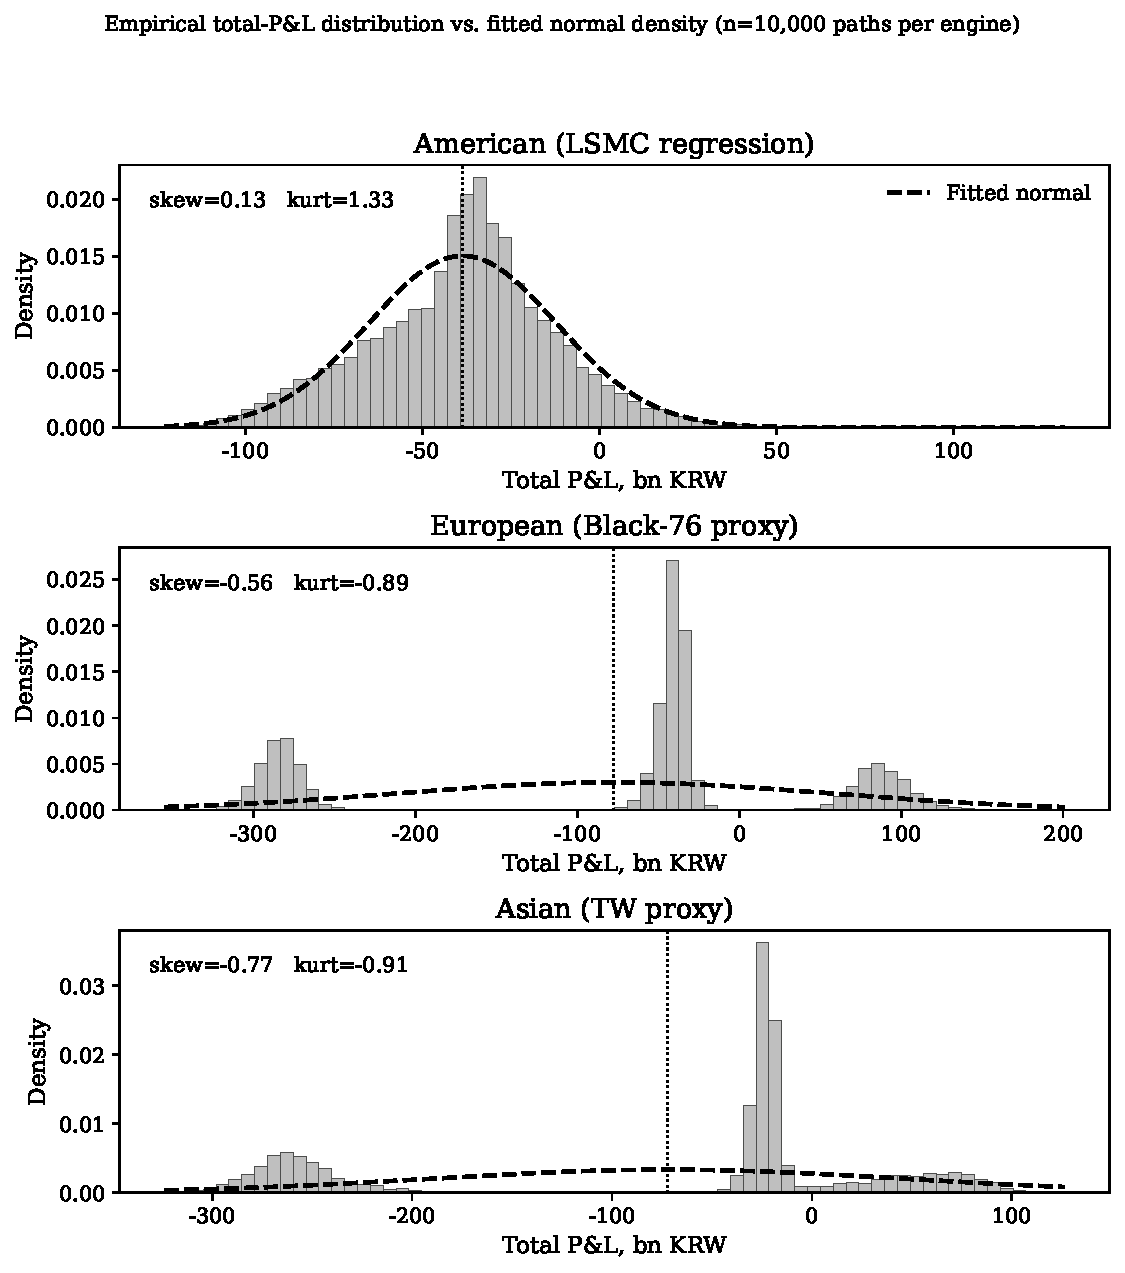
\includegraphics[height=0.46\textheight,keepaspectratio]{figures/fig_pl_distribution.pdf}
\caption{Empirical total-P\&L distribution (gray histogram) vs.\ a normal density fitted to the same mean and standard deviation (black dashed), by engine.}
\label{fig:pldist}
\end{figure}

The contrast is stark. American's total-P\&L distribution is unimodal and only mildly non-normal (skewness $0.13$, excess kurtosis $1.33$); both proxy engines are \emph{trimodal} at a default kernel bandwidth, with a severe-loss cluster near $-$KRW 280---300 billion, a moderate-loss cluster, a smaller gain cluster. Their failure of normality is not tail thickness (both are mildly platykurtic, $-0.89$ and $-0.91$) but multimodality: three sub-populations sorted by which of the barrier, the FX co-movement, and the (absent) barrier-aware delta protection each path realizes. A proxy delta does more than add noise: it produces a categorically different, multi-regime P\&L distribution that its own mean and standard deviation cannot summarize. The modality claim is bandwidth-sensitive and is reported as such: a Gaussian kernel density on the proxy ledger at Scott's default bandwidth resolves three local maxima, near KRW $-252$bn, $-130$bn and $+2$bn, but widening the bandwidth by a factor of two collapses these to two and by a factor of three to one. The distribution is therefore broad and left-skewed (skew $-1.39$, excess kurtosis $+0.35$) with structure at the default resolution, and the paper does not claim a formally tested multimodality; no dip test is reported.

\subsection{Alive-and-In-the-Money Path Density}
\label{sec:itmdecay}

The regression's step-wise reliability depends on the alive-and-ITM path count. Figure \ref{fig:itmdecay} reports that fraction by elapsed time across six maturities: from a life-mean of $45.7\%$ at $0.5$ years down to $18.9\%$ at $3.0$ years, with the $3.0$-year structure's terminal fraction at just $3.0\%$, the mechanical reason regression reliability degrades with maturity (Section~\ref{sec:fdcheck}).

\begin{figure}[h]
\centering
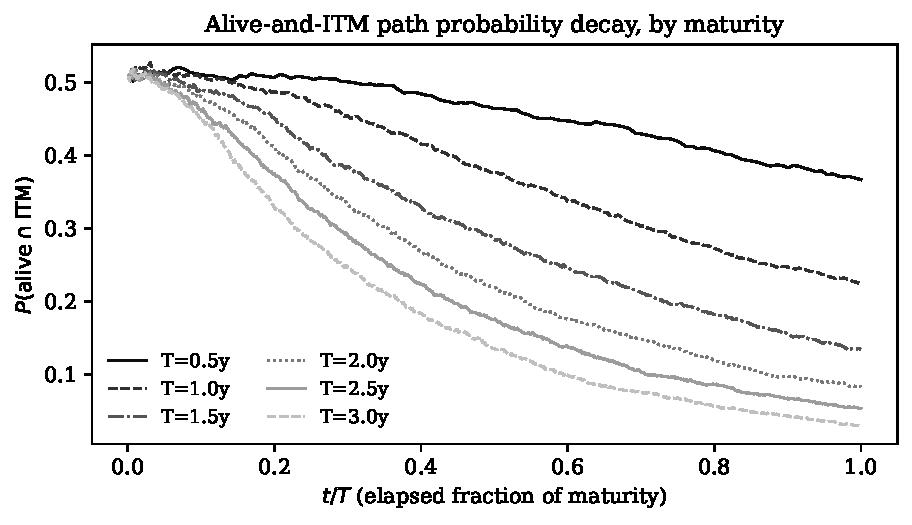
\includegraphics[width=0.72\textwidth]{figures/fig_itm_alive_decay.pdf}
\caption{Alive-and-ITM path probability by elapsed time fraction, across six tested maturities.}
\label{fig:itmdecay}
\end{figure}

\section{Sensitivity Studies}
\label{sec:sensitivity}

\subsection{Finite-Difference vs.\ Regression Delta}
\label{sec:fdcheck}

Table \ref{tab:deltacheck} and Figure \ref{fig:deltacheck} compare the closed-form LSMC regression delta of Section~\ref{sec:delta} against an independent finite-difference (bump-and-reprice) delta computed by re-running the full LSMC pricer at $S_1(0)\pm\varepsilon$, at three points across the structure's life.

\begin{table}[h]
\centering
\caption{Finite-difference vs.\ regression delta, WTI leg. Both columns re-measured on the exact engine at $100{,}000$ paths per replication over five independent seeds; standard deviations across seeds in parentheses. The finite difference is a central bump-and-reprice at $\varepsilon=5\%$ with the contract strike \emph{held fixed} at $K=78.94$ while the spot is bumped, which is the sensitivity a hedging desk needs.}
\label{tab:deltacheck}
\begin{tabular}{lrrrr}
\toprule
$t/T$ & FD delta & Regression delta & Abs.\ diff.\ & \% of FD \\
\midrule
0.00 & 0.5342 (0.0055) & 0.5759 (0.0772) & 0.0417 & $7.8\%$ \\
0.50 & 0.5457 (0.0066) & 0.6999 (0.0200) & 0.1542 & $28.3\%$ \\
0.90 & 0.5355 (0.0010) & 0.9232 (0.0361) & 0.3877 & $72.4\%$ \\
\bottomrule
\end{tabular}
\end{table}

\begin{figure}[h]
\centering
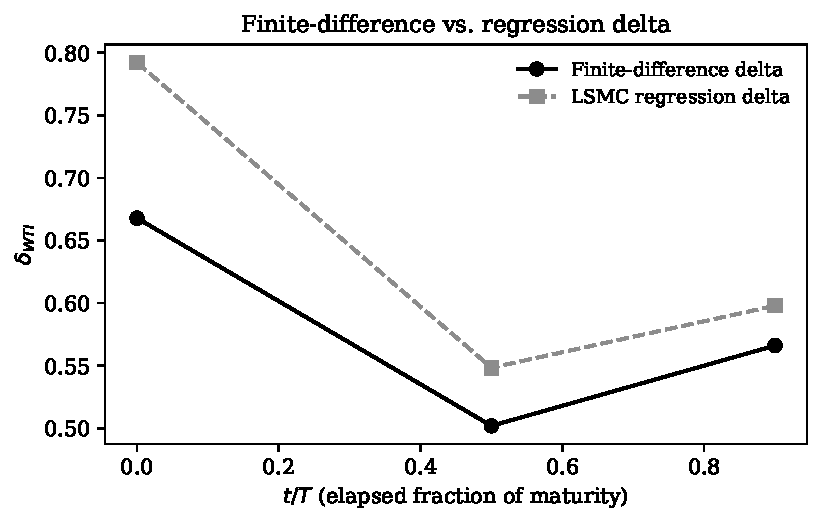
\includegraphics[width=0.62\textwidth]{figures/fig_delta_check.pdf}
\caption{Finite-difference delta vs.\ LSMC regression delta, by elapsed time fraction.}
\label{fig:deltacheck}
\end{figure}

The re-measured gap is modest at inception and widens with elapsed time: $7.8\%$ at $t/T=0$, $28.3\%$ at mid-life and $72.4\%$ at $t/T=0.9$. Two things about the measurement are worth stating, because an earlier version of this section got both wrong.

First, the bump must hold the contract strike fixed. Bumping the spot while letting $K$ follow it measures the sensitivity of a permanently at-the-money contract to a joint translation of spot and strike, which is a different object and, on this structure, roughly an order of magnitude smaller. Table~\ref{tab:deltacheck} holds $K=78.94$ throughout. Second, with the strike fixed the price is monotone increasing in spot over $S_1(0)\in[71,103]$, with an average slope of $0.58$; the barrier at $U=120$ does not turn the value over inside that range at a ten-month horizon.

The direction of the remaining gap is the informative part. The regression delta is close to the finite difference early, when the option is at the money and the barrier is far, and drifts above it as the option ages: by $t/T=0.9$ it reads $0.92$ against a measured $0.54$. This is the opposite of the profile a converging estimator would show, and it is consistent with what Section~\ref{sec:awareness} documents below, namely that the fitted surface has very little state dependence at all. The finite-difference side is the tightly determined one throughout, with a seed standard deviation of $0.006$ or less; the regression side carries a seed dispersion of $0.077$ at inception, which Section~\ref{sec:awareness} traces to a rank-deficient first-step design matrix.

The consequence for the rest of the paper is bounded. The hedge-cost comparisons of Section~\ref{sec:hedgecost} compare two hedging \emph{rules} applied to identical paths and do not require either delta to be an accurate price sensitivity. Any use of the regression gradient as $\partial V/\partial S_1$, on the other hand, carries an error that grows from under ten percent at inception to more than seventy percent near expiry, and a desk sizing from it late in the option's life would over-hedge accordingly.

\subsection{How much state dependence does the surface have?}
\label{sec:awareness}

The level comparison above says the surface is close to correct early and drifts high late. A sharper question is whether it varies with the state at all. Table~\ref{tab:aware} compares the surface delta with the barrier-blind Black-76 delta by moneyness bucket at mid-life, on a common $100{,}000$-path bank restricted to in-the-money survivors.

\begin{table}[h]
\centering
\small
\begin{tabular}{lrrr}
\toprule
WTI bucket & nodes & surface $\delta$ & Black-76 $\delta$ \\
\midrule
$[79,\,85)$   & 11{,}102 & 0.7087 & 0.6003 \\
$[92,\,100)$  &  9{,}005 & 0.6958 & 0.8318 \\
$[115,\,120)$ &     522 & 0.6761 & 0.9592 \\
\bottomrule
\end{tabular}
\caption{Regression-surface delta against the Black-76 delta by moneyness at $t/T=0.5$. The surface delta spans $0.033$ across the entire in-the-money domain; the Black-76 delta spans $0.36$.}
\label{tab:aware}
\end{table}

The result is negative and it should be reported as such. Across the whole in-the-money domain the surface delta moves by $0.033$, from $0.709$ just above the strike to $0.676$ within five dollars of the barrier, while the Black-76 delta moves by $0.36$ over the same range. The surface is a constant plus fitting noise. Its apparent ``damping'' near the barrier, $0.676$ against Black-76's $0.959$, is not damping: just above the strike the same surface reads $0.709$ against Black-76's $0.600$, high by the same order and in the wrong direction. A genuine up-and-out delta rises with moneyness and then collapses toward and through zero as the barrier approaches; this one does neither.

Two further diagnostics complete the picture. Over $17{,}342{,}543$ hedged nodes the raw delta never turns negative, with a minimum of $+0.357$ and $+0.582$ within ten percent of the upper barrier, so the $\mathrm{clip}_{[0,1]}$ of Section~\ref{sec:delta} never binds below; the upper clip binds on $1.42\%$ of nodes, and removing the clip entirely leaves the hedge-cost mean unchanged and moves the standard deviation from KRW $51.25$bn to $51.27$bn. And at the first step the design matrix is badly conditioned, $\mathrm{cond}(X'X)\approx1.8\times10^{10}$ against the solver's $\mathrm{rcond}=10^{-10}$, because $v_1$ and $v_2$ carry one day of cross-sectional dispersion; the fitted coefficients there are an order of magnitude larger than from step 20 onward and nearly cancel, which is the source of the inception seed dispersion and of the sign instability in $\partial V/\partial S_2$ discussed in Section~\ref{sec:limitations}.

The honest summary is therefore narrower than this paper's earlier drafts claimed. The five-term surface is not a barrier-aware delta estimator in any strong sense: it is close to a constant over the fitted domain, it does not reproduce the barrier's characteristic sign reversal, and it is poorly conditioned at inception. What Section~\ref{sec:hedgecost} measures is the performance of the \emph{hedging rule} it induces on a common path bank, and Section~\ref{sec:limitations} sets out what that comparison can and cannot support.

\subsection{Hedge-Cost Sensitivity to the FX Coupling Multiplier}
\label{sec:fxsweep}

The one-parameter coupling $\delta_{FX}=c\cdot\delta_{WTI}$, evaluated at the natural reference point $c=1.0$, is tested directly by sweeping $c\in\{0.5,0.75,1.0,1.25,1.5\}$ and holding the WTI delta strategy fixed. Table \ref{tab:fxsweep} and Figure \ref{fig:fxsweep} report the results; note that the KO rate ($0.2249$) and early-exercise rate ($0.4551$) are, as expected, identical across every value of $c$, since $c$ only rescales the FX leg and has no influence on the WTI-side stopping decisions, so any change in cost or variance across the sweep is attributable purely to the FX-leg coupling, not to a change in the underlying barrier or exercise behavior.

\begin{table}[h]
\centering
\caption{FX hedge multiplier sweep, total P\&L, KRW}
\label{tab:fxsweep}
\begin{tabular}{lrrrr}
\toprule
$c$ & Mean total P\&L & Std.\ total P\&L & VaR$_{95}$ & CVaR$_{95}$ \\
\midrule
0.50 & $-43{,}617{,}209{,}156$ & $32{,}187{,}496{,}866$ & $121{,}445{,}143{,}908$ & $131{,}417{,}052{,}157$ \\
0.75 & $-49{,}682{,}343{,}643$ & $44{,}990{,}807{,}824$ & $184{,}328{,}803{,}921$ & $195{,}166{,}753{,}028$ \\
1.00 & $-55{,}747{,}478{,}129$ & $59{,}369{,}149{,}552$ & $247{,}282{,}335{,}313$ & $259{,}001{,}910{,}328$ \\
1.25 & $-61{,}812{,}612{,}616$ & $74{,}415{,}081{,}430$ & $310{,}081{,}379{,}678$ & $322{,}907{,}477{,}949$ \\
1.50 & $-67{,}877{,}747{,}102$ & $89{,}793{,}641{,}566$ & $372{,}580{,}157{,}785$ & $386{,}866{,}592{,}247$ \\
\bottomrule
\end{tabular}
\end{table}

\begin{figure}[h]
\centering
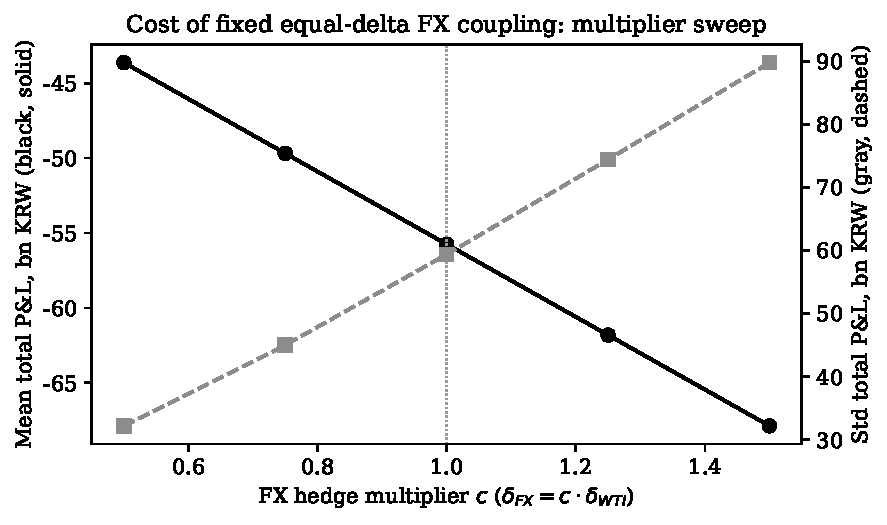
\includegraphics[width=0.68\textwidth]{figures/fig_delta_fx_sweep.pdf}
\caption{Total P\&L mean and standard deviation as a function of the FX hedge multiplier $c$.}
\label{fig:fxsweep}
\end{figure}

Within the swept range, both the mean total P\&L and its standard deviation are monotonic in $c$: variance is smallest, and mean P\&L least negative, at the smallest tested multiplier $c=0.5$, and both deteriorate steadily through $c=1.5$. This shows the natural reference point $c=1.0$ is neither a risk-minimizing anchor nor even a neutral midpoint: it sits on the costly end of a clear, monotone trade-off, and every step toward a smaller FX multiplier makes the hedge cheaper and less volatile over this range. The mechanism is structural: because $c$ scales the FX notional in lock-step with the WTI delta regardless of the FX leg's own volatility, correlation, and moneyness, the coupling forces the FX leg to carry more notional than its own risk profile would independently justify once $c$ approaches and exceeds $1.0$. The monotone direction is enough to establish that sizing the FX leg as a fixed multiple of the WTI delta is a source of avoidable hedging cost whenever the multiple is not chosen with the two legs' covariance in mind; the next two subsections turn that direction into the actual minimizer, first within the coupled family (a closed-form, covariance-aware optimal multiplier), then for the instrument-free question of what the FX delta \emph{should} be (the structure's own analytic FX sensitivity).

\subsection{From sweep to minimizer: the closed-form optimal multiplier}
\label{sec:cstar}

The five-point sweep is a sampling of a curve whose exact shape is fixed by the engine's structure. At every rebalancing date the FX position enters the ledger only through $\delta_{FX}=c\cdot\delta_{WTI}$; the WTI leg, the barrier stopping rule, and the early-exercise decision are all computed from the WTI surface alone and are therefore untouched by $c$ (this is why the KO and exercise rates in Table~\ref{tab:fxsweep} are invariant across the sweep). Consequently the cumulative FX-leg cash flow scales linearly in $c$ path by path, and the per-path hedge cost decomposes affinely:
\begin{equation}
\label{eq:hcaffine}
\mathrm{HC}_p(c) = A_p + c\,B_p, \qquad A_p = \mathrm{HC}_p(0), \quad B_p = \mathrm{HC}_p(1)-\mathrm{HC}_p(0),
\end{equation}
where $A_p$ is the WTI-leg-only hedge cost (FX coupling switched off) and $B_p$ is the unit FX-leg contribution, both recovered from just two engine runs ($c=0$ and $c=1$) by per-path differencing. The mean is therefore affine in $c$ with no interior optimum, which is precisely why the swept mean is monotone, and the variance is an exact upward parabola,
\begin{equation}
\label{eq:hcvar}
\mathbb E[\mathrm{HC}(c)] = \mathbb E[A]+c\,\mathbb E[B], \qquad
\mathrm{Var}[\mathrm{HC}(c)] = \mathrm{Var}[A] + 2c\,\mathrm{Cov}(A,B) + c^2\,\mathrm{Var}[B],
\end{equation}
whose unique minimizer is a one-line quotient, structurally Ederington's (1979) univariate minimum-variance hedge ratio, with $A$ as the exposure and the unit FX leg $B$ as the hedging instrument:
\begin{equation}
\label{eq:cstar}
c^\star = -\frac{\mathrm{Cov}(A,B)}{\mathrm{Var}[B]}, \qquad
\mathrm{Var}[\mathrm{HC}(c^\star)] = \mathrm{Var}[A]\bigl(1-\rho_{A,B}^2\bigr).
\end{equation}
The swept range $[0.5,1.5]$ is simply the right arm of this parabola, which is why cost variance rises monotonically across it: the vertex lies to the \emph{left} of the entire tested window.

One qualification is essential to reading $c^\star$ correctly, and it concerns what is being minimized. In Ederington's setting $A$ is the firm's \emph{spot exposure}. Here $A=\mathrm{HC}_p(0)$ is the WTI leg's own hedge cost, so \eqref{eq:hcvar} is the variance of the \emph{hedging programme's ledger}, not of the firm's total position: the importer's physical exposure, $\$157{,}880{,}000$ of monthly dollar settlement against $2{,}000{,}000$ barrels, appears in neither $A$ nor $B$. This is why $c^\star$ can come out negative. A negative FX delta means shorting the currency leg, which reduces the dispersion of the hedge ledger while \emph{increasing} the dollar exposure of a firm that is already structurally long USD. The two objectives are different, and on this structure they disagree in sign. A treasury minimizing total-P\&L variance, with the physical exposure written into $A$, would obtain a different and plausibly positive multiplier; the number reported here answers the narrower question of how to size the FX leg so that the option book's own cost is least volatile. Section~\ref{sec:structdelta}'s $V/S_2$ is subject to the same reading: it is the FX sensitivity of the option position, which is the quantity a dealer marking that position hedges, and not the FX exposure of the importer's underlying purchase programme.

Equation~\eqref{eq:hcaffine} is an identity forced by the engine: a third run at $c=0.5$ reproduces $A_p+0.5\,B_p$ path by path with maximum relative error below $10^{-15}$. On that re-implementation at $n=200{,}000$ jump-adapted exact paths (Section~\ref{sec:rigor}; the same 217-step daily grid, WTI surface fitted by least-squares Monte Carlo on the full path bank), the minimizer is
\begin{equation}
c^\star = -0.548 \quad (\text{stable across hedge seeds at smaller } n,\ \text{range } [-0.56,\,-0.52]),
\end{equation}
a \emph{negative} multiplier: the covariance $\mathrm{Cov}(A,B)$ is positive, so a positively-coupled FX leg adds cost variance that co-moves with the WTI-leg cost and not offsetting it, and the variance-minimizing FX position runs opposite to the full-pass-through direction. Because $\mathbb E[B]>0$ (the FX leg costs premium on average), the affine mean~\eqref{eq:hcvar} is lower at $c^\star$ than at $c=1$ as well, so $c^\star$ improves both moments relative to the reference point simultaneously. What it improves them by, however, is modest: hedge-cost standard deviation falls from KRW $51.90$ billion at $c=1$ to KRW $48.76$ billion at $c^\star$, a reduction of only about $6\%$. The FX coupling is thus a genuine but second-order lever on hedge-cost risk: the WTI leg dominates the variance $\mathrm{Var}[A]$, and no choice of $c$ can touch that part. This is the dynamic-hedging counterpart of the static allocation finding that the FX leg optimally carries only a few percent of coverage: the two analyses reach the same qualitative verdict on the FX leg's small role from entirely separate objectives.

\begin{figure}[htbp]
\centering
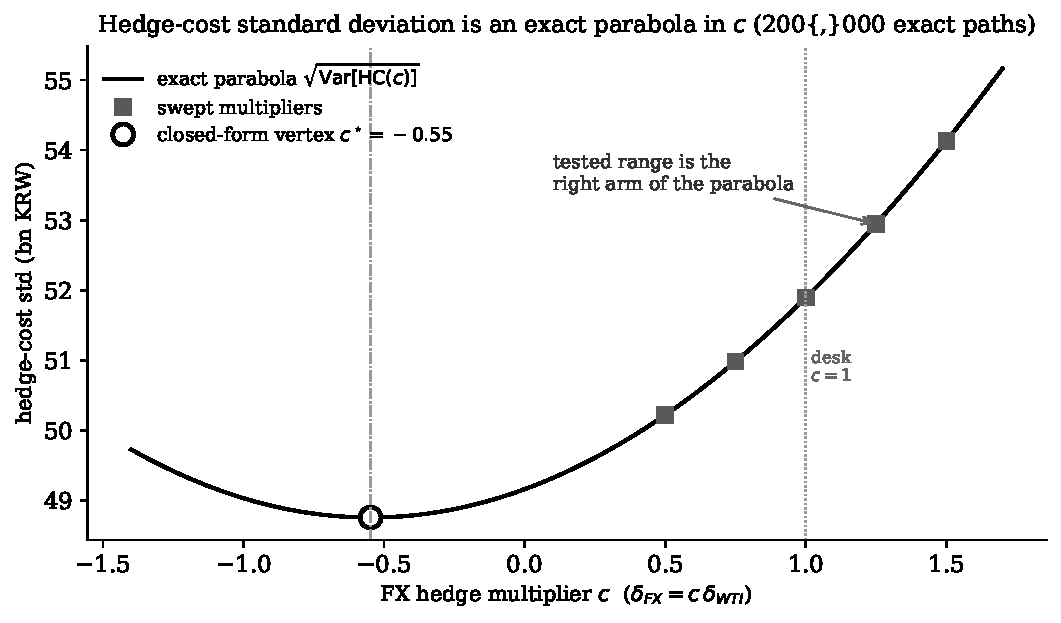
\includegraphics[width=0.78\textwidth]{figures/fig_cstar_parabola.pdf}
\caption{Hedge-cost standard deviation as the exact parabola $\sqrt{\mathrm{Var}[\mathrm{HC}(c)]}$ implied by the affine decomposition~\eqref{eq:hcaffine}, computed at $200{,}000$ jump-adapted exact paths (Section~\ref{sec:rigor}). The five swept multipliers (Table~\ref{tab:fxsweep}) lie on the parabola's right arm; the natural reference point $c=1$ sits well up that arm, and the closed-form vertex $c^\star=-0.55$~\eqref{eq:cstar}, the variance minimizer, lies to the left of the entire tested range.}
\label{fig:cstar}
\end{figure}

Hedge-cost standard deviation at $c=1$ is KRW $51.90$ billion with a unimodal P\&L shape, and the early-exercise rate runs high (Section~\ref{sec:limitations} isolates the cause to the fitted continuation-value surface, not to path discretization), shifting the mean, so $c^\star$'s exact value is re-implementation-derived, while the closed form~\eqref{eq:cstar} and the affine identity~\eqref{eq:hcaffine} are structural and independent of that gap.

\subsection{What the FX delta should be: the structure's own analytic sensitivity}
\label{sec:structdelta}

The multiplier $c^\star$ answers the best-scalar question \emph{within} the coupled family $\delta_{FX}=c\,\delta_{WTI}$, but a coupled family is itself only one way to size the FX leg, so the deeper question is what the FX hedge ratio would be if it were not tied to $\delta_{WTI}$ at all. For this structure that question has an exact answer. The quanto payoff, its double barrier, and its jump component all act on $S_1$ alone; the exchange rate $S_2$ enters only as a multiplicative terminal factor. Writing the option value $V(t)=\mathbb E_t^{\mathbb Q}[\,\mathbf 1\{\tau_{KO}>T\}\max(S_1(T)-K,0)\,S_2(T)\,]$ and separating the $S_2$ factor by the standard exponential-martingale (quanto) argument,
\begin{equation}
\label{eq:homog}
V(t) = S_2(t)\,g\bigl(S_1(t),\ \text{path-state},\ t\bigr),
\end{equation}
exactly linear in $S_2(t)$: the $S_2$ factor pulls out of the expectation as $S_2(t)e^{(r_{KRW}-r_{US})\tau}$ while the tilt shifts $S_1$'s drift by the quanto term $\rho\sigma_1\sigma_2$ and leaves the barrier, the jumps, and (since both continuation and exercise values are linear in $S_2$) the early-exercise region untouched. Homogeneity of degree one in $S_2$ gives the structural FX delta in closed form,
\begin{equation}
\label{eq:structdelta}
\delta_{FX}^{\mathrm{struct}}(t) \;=\; \frac{\partial V}{\partial S_2} \;=\; \frac{V(t)}{S_2(t)},
\end{equation}
i.e.\ the option's true FX exposure is precisely its own USD value, and \emph{not} a scalar multiple of $\delta_{WTI}$ times the (far larger) barrel notional a coupled rule sizes it against. This is the analytic root of the sweep's cost: a coupled rule sizes the FX hedge off the WTI hedge notional $\min(S_1,K)\cdot\text{barrels}$, whereas the exposure that actually needs hedging is the option's own carrying value $V$. Reconciled to a common unit, the coupled family's FX position at $c=1$ carries a median USD notional of roughly $4.6$ times the structural requirement of Eq.~\eqref{eq:structdelta}, which at the reported premium is an option carrying value of about \$22.2M against a coupled position near \$102M. The comparison is stated as a notional ratio rather than a contract count because the ratio is invariant to the futures contract size a given desk trades, while the count is not: a one-for-one coupling over-hedges the FX leg by roughly $4.6\times$.

Two internal cross-checks accompany this. First, the fitted regression surface provides a second, independent estimate of the same delta, $\partial\tilde V/\partial S_2 = (\beta_2+2\beta_4 v_2+\beta_5 v_1)/S_2(0)$, computed from the very coefficients that price the option (Section~\ref{sec:delta}); it agrees with the homogeneity form $V/S_2$ to a median $8.8\%$ over the surface, so the fitted basis respects the structure's known $S_2$-linearity to within that gap and the residual is a measurable property of the five-term polynomial and not of the theorem, which is exact. Second, and more striking, the structural delta~\eqref{eq:structdelta} is \emph{positive} (long FX, since the option's KRW value rises with the exchange rate), whereas the variance-minimizing multiplier $c^\star$ of Section~\ref{sec:cstar} is \emph{negative}: the two disagree not only in size but in sign, because they answer different questions. Equation~\eqref{eq:structdelta} hedges the option's mark-to-market FX exposure; $c^\star$ minimizes the variance of the running hedge \emph{cost}, a quantity dominated by the WTI-leg futures P\&L with which a positively-coupled FX leg happens to co-move. Any single coupled scalar $\delta_{FX}=c\,\delta_{WTI}$ conflates these two objectives, and at the natural reference point $c=1$ serves neither, since it neither matches the structural FX exposure~\eqref{eq:structdelta} nor sits near the cost-variance minimizer $c^\star$.

\subsection{Jump Risk-Premium Re-Pricing Sensitivity}
\label{sec:jumpsens}

Table \ref{tab:jumpsens} and Figure \ref{fig:jumpsens} report how the base and stress premiums respond to a pure re-pricing sweep of the risk-neutral jump intensity $\lambda_Q$, holding jump-size distribution parameters fixed. This is explicitly \emph{not} a Girsanov jump-measure change; a fully self-consistent jump-measure transformation requires an Esscher transform applied jointly to both the jump intensity and the jump-size distribution to remain risk-neutral, which is outside the scope of the diagnostic reported here.

\begin{table}[h]
\centering
\caption{Jump-intensity re-pricing sweep}
\label{tab:jumpsens}
\begin{tabular}{lrrr}
\toprule
$\lambda_Q$ factor & $\lambda_Q$ (per year) & Base premium & Stress premium \\
\midrule
1.00 & 6.7846 & 17{,}188.10 & 52{,}507.01 \\
1.25 & 8.4808 & 17{,}743.27 & 52{,}263.00 \\
1.50 & 10.1769 & 18{,}207.37 & 52{,}234.79 \\
2.00 & 13.5692 & 19{,}009.40 & 51{,}974.72 \\
\bottomrule
\end{tabular}
\end{table}

\begin{figure}[h]
\centering
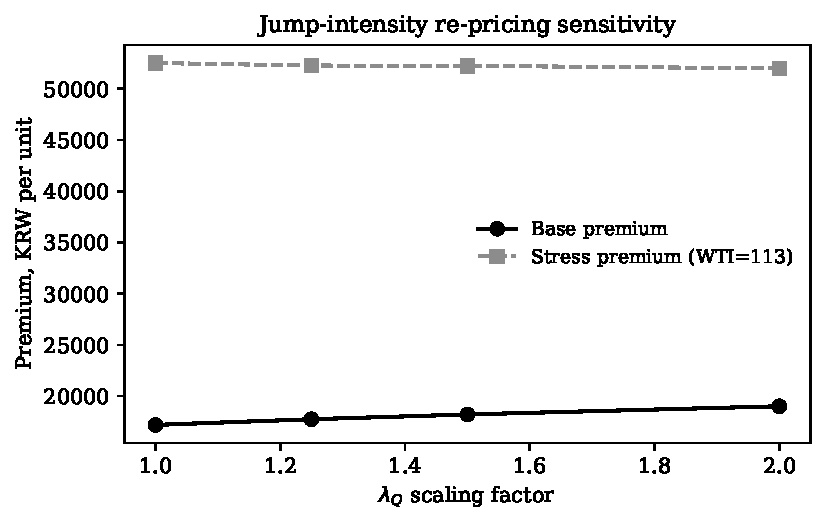
\includegraphics[width=0.62\textwidth]{figures/fig_jump_premium_sensitivity.pdf}
\caption{Base and stress premium as a function of the jump-intensity re-pricing factor.}
\label{fig:jumpsens}
\end{figure}

The base premium rises monotonically with $\lambda_Q$, as expected: a higher priced-in jump intensity raises the expected cost of a claim exposed to jump risk. The stress premium (computed under the WTI $=113$ scenario, with all other inputs at the Table~\ref{tab:asymjump} calibration) moves in the opposite direction, falling slightly as $\lambda_Q$ rises. The direction is consistent with the mechanism: under a deep-stress, near-certainly-ITM scenario the option's value is dominated by intrinsic value and not optionality, so raising the priced-in jump risk (which primarily inflates the value of the \emph{optionality} component) has a comparatively small, and in this case slightly negative, effect once intrinsic value already dominates the payoff. Note also that this sweep's own $\lambda_Q$-factor-1.0 base premium of KRW $17{,}188.10$ differs from the headline production base premium of KRW $17{,}132.47$ (Section~\ref{sec:baseline}) by roughly $0.32\%$, an independently reseeded Monte Carlo draw of the same underlying model, and a useful empirical read on the baseline premium's own Monte Carlo standard error.

\subsection{Jump-Threshold Calibration Robustness}
\label{sec:lambdarob}

Table \ref{tab:lambdarob} and Figure \ref{fig:lambdarob} report how the fitted jump parameters, KO rate, and total P\&L moments respond to varying the jump-classification threshold $k$ (in multiples of $\sigma\sqrt{dt}$) used by the calibration engine's threshold-based jump identification heuristic (Section~\ref{sec:calibration}), holding the historical return series fixed. This sweep runs on the same jump-adapted exact engine and the same $n=200{,}000$ path count as Section~\ref{sec:rigor}. Its KO-rate column is \emph{not} on the same definition as Section~\ref{sec:baseline}'s: the calibration sweep re-fits $(\lambda,\sigma_1)$ at each threshold and re-prices on a re-struck grid, and the resulting rates ($0.171$--$0.174$) are accordingly a factor of roughly $2.5$ below the baseline barrier-touch frequency of $0.4369$ and cannot be read against it. What the column supports is the \emph{within-sweep} comparison across $k$, which is the only claim made from it; the same caveat applies to the total-P\&L moments in the two right-hand columns, which sit on a different configuration from Table~\ref{tab:hedgecost} and should likewise be read only across rows.

\begin{table}[h]
\centering
\caption{$k$-sigma threshold robustness sweep}
\label{tab:lambdarob}
\begin{tabular}{lrrrrr}
\toprule
$k$ & $\lambda$ (per year) & Base premium & KO rate & Mean total P\&L & Std.\ total P\&L \\
\midrule
2.5 & 15.714 & 17{,}610.40 & 0.1744 & $-54{,}965{,}034{,}614$ & $64{,}303{,}604{,}528$ \\
3.0 & 6.7898 & 17{,}481.98 & 0.1727 & $-56{,}161{,}658{,}548$ & $66{,}183{,}065{,}596$ \\
3.5 & 3.686 & 17{,}455.32 & 0.1711 & $-54{,}951{,}253{,}711$ & $64{,}795{,}934{,}047$ \\
\bottomrule
\end{tabular}
\end{table}

\begin{figure}[h]
\centering
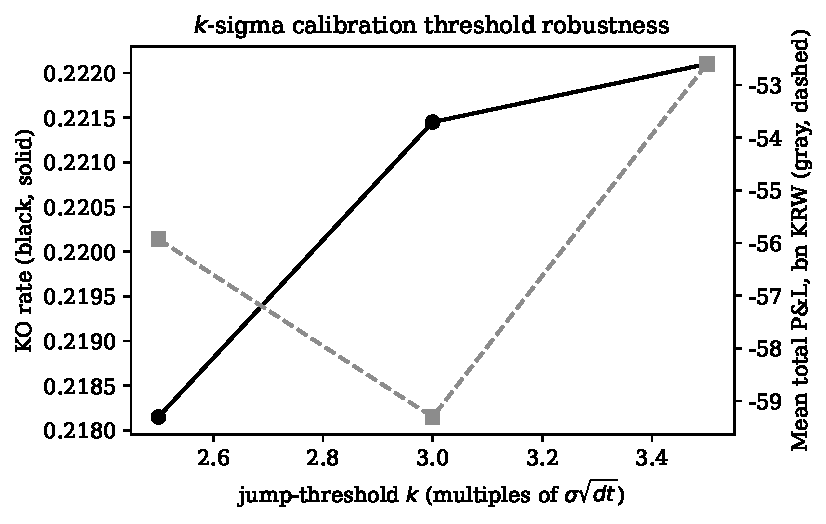
\includegraphics[width=0.62\textwidth]{figures/fig_lambda_robustness.pdf}
\caption{KO rate and mean total P\&L as a function of the jump-classification threshold $k$.}
\label{fig:lambdarob}
\end{figure}

The fitted jump intensity is highly sensitive to $k$: a looser threshold ($k=2.5$) classifies more than four times the jump frequency of a tighter one ($k=3.5$), $15.7$ versus $3.7$ jumps per year, as diffusive moves get reclassified as jumps. Despite this range in fitted $\lambda$, the base premium moves by under $1\%$ and the KO rate stays essentially flat ($0.171$---$0.174$), because the EM-style calibration re-solves the diffusive volatility to compensate for whatever variance the threshold assigns to jumps instead, total variance is conserved across the split, and price and barrier behavior inherit that conservation. The $k=3.0$ row's $\lambda=6.7898$ and the production baseline's $\lambda=6.7846$ are the same threshold-count estimator evaluated on samples differing by one observation, $35\times252/1299$ against $35\times252/1300$. They are not two independent methods, and their agreement is arithmetic rather than evidential; the informative content of this sweep is the variation \emph{across} $k$, not the agreement at $k=3$.

\section{Model Validation and Robustness}
\label{sec:pqval}

\subsection{Exact Validation: Closed-Form Drift Bias}
\label{sec:exactval}

The simplest test of the orthogonal Girsanov construction (Section~\ref{sec:girsanov}) compares its closed-form predicted drift bias against the same bias measured directly by simulation, for a family of simple (non-path-dependent, non-barrier) test statistics, across a range of maturities and a range of market-price-of-risk scalings. Table \ref{tab:driftbias} reports the maturity sweep.

\begin{table}[h]
\centering
\caption{Closed-form vs.\ simulated drift bias, by maturity}
\label{tab:driftbias}
\begin{tabular}{S[table-format=1.1] S[table-format=-2.4] S[table-format=-2.4] S[table-format=-1.1e-2,exponent-product=\times,retain-explicit-plus=false]}
\toprule
{$T$ (years)} & {Simulated bias} & {Theoretical bias} & {Residual} \\
\midrule
0.5 & -17.5777 & -17.5777 & 7.1e-15 \\
1.0 & -27.6171 & -27.6171 & 3.6e-14 \\
1.5 & -32.2205 & -32.2205 & 2.3e-13 \\
2.0 & -35.7635 & -35.7635 & 2.1e-13 \\
2.5 & -35.0405 & -35.0405 & -1.1e-13 \\
3.0 & -37.2824 & -37.2824 & 4.3e-14 \\
\bottomrule
\end{tabular}
\end{table}

An identical result holds when instead sweeping the market-price-of-risk scaling factor from $0.5\times$ to $1.5\times$ the baseline $\mu^{\mathbb P}$, with simulated bias again matching the theoretical closed form. Both sweeps confirm the orthogonal Girsanov construction of Section~\ref{sec:girsanov} is implemented correctly at the level of raw drift moments: this is an exact test in the sense that no discretization error, path-dependent payoff, or barrier feature is involved, only the correctly-orthogonalized first-moment shift itself.

\subsection{Inexact Validation: Reweighting the Actual Barrier Payoff}
\label{sec:inexactval}

A stronger test reweights genuinely simulated $\mathbb Q$-measure paths, carrying the barrier-monitored KO structure's actual payoff, by the Girsanov likelihood ratio $L(T)$, and compares the resulting reweighted mean payoff against a direct $\mathbb P$-measure simulation of the same payoff under the true physical drift. Table \ref{tab:girsanov} and Figure \ref{fig:girsanov} report the result.

\begin{table}[h]
\centering
\caption{Girsanov reweighting vs.\ direct simulation, KO payoff}
\label{tab:girsanov}
\begin{tabular}{lrr}
\toprule
Method & Mean payoff & Std.\ dev.\ payoff \\
\midrule
Reweighted ($\mathbb Q$-paths $\times$ Girsanov LR) & 6{,}224.31 & 14{,}346.47 \\
Direct ($\mathbb P$-measure simulation) & 6{,}217.66 & 12{,}782.30 \\
\midrule
Residual (mean difference) & \multicolumn{2}{r}{6.65} \\
Residual (\% of direct mean) & \multicolumn{2}{r}{$+0.11\% \pm 0.10$} \\
\bottomrule
\end{tabular}
\end{table}

\begin{figure}[h]
\centering
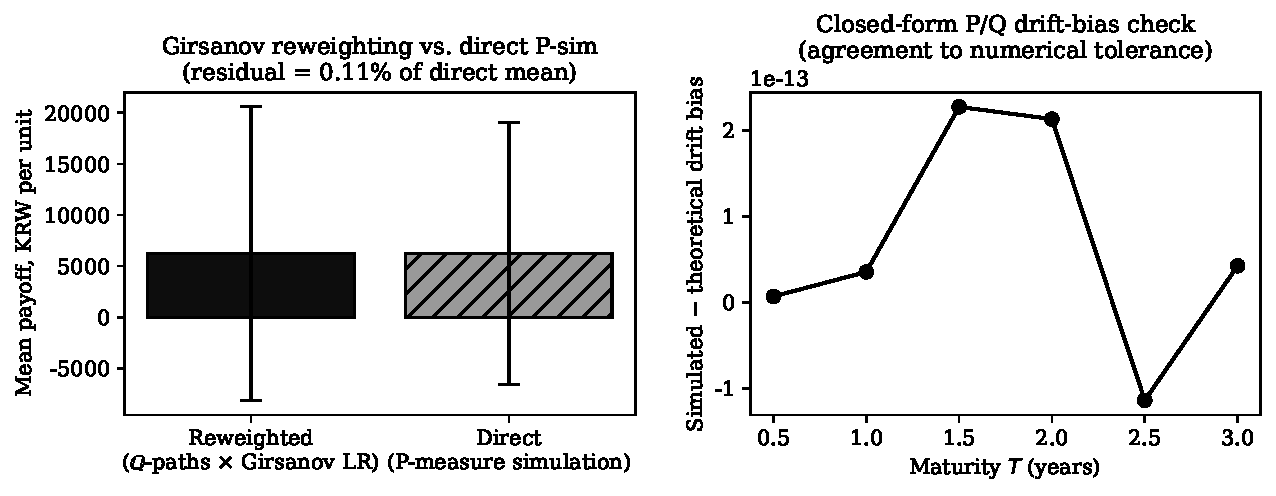
\includegraphics[width=0.92\textwidth]{figures/fig_girsanov_validation.pdf}
\caption{Left: Girsanov-reweighted vs.\ direct-simulation mean payoff on the actual KO structure. Right: agreement of the corresponding closed-form drift-bias test to within numerical tolerance (Table \ref{tab:driftbias}).}
\label{fig:girsanov}
\end{figure}

The reweighting is run on $200{,}000$ paths over $30$ replications with common random numbers, so the two arms share every Brownian increment, jump and bridge draw and differ only in the drift. The residual is $+0.11\%$ with a standard error of $0.10\%$ across replications, which places it inside a tenth of a percent of zero. The density that does the reweighting is checked directly on the same runs: $\mathbb E[L] = 1.000022$ and $\mathrm{sd}[L] = 0.284216$ against the closed form $\sqrt{e^{\theta^2 T}-1} = 0.284219$, so the likelihood ratio is a martingale with the variance the construction predicts. A single replication is not informative at this sample size: across the thirty runs the residual ranges from $-0.78\%$ to $+1.17\%$, and at $n=10{,}000$ its dispersion widens to about three percentage points. The two tests differ in the property that matters: Section~\ref{sec:exactval}'s test statistics are smooth, low-order moments of the underlying diffusion with no discretization-sensitive discontinuity, whereas the KO payoff tested here is a genuinely discontinuous function of the path (it depends on whether a discrete barrier-touch event occurred at all, evaluated on a finite, 217-step Euler---Maruyama discretization of a continuous-time process). Reweighting by a likelihood ratio is a variance-amplifying operation in general (note the reweighted standard deviation ($14{,}346$) exceeds the direct standard deviation ($12{,}782$) by roughly $12\%$ in Table \ref{tab:girsanov}), and that amplified variance, combined with the barrier discontinuity's own discretization error (Section~\ref{sec:bridge}), is sufficient to produce a residual of this size without any defect in the measure-change construction itself. For a reweighted discontinuous barrier payoff at this sample size, a residual indistinguishable from zero would itself have warranted scrutiny.

\subsection{Exact Simulation, Error Decomposition, and Convergence}
\label{sec:rigor}

The production scheme (Euler steps, whole-step bridge on jump-free steps) carries three approximation layers: diffusion discretization, the bridge's jump-blindness (Eq.~\ref{eq:jumpgap}), and Monte Carlo noise. This section eliminates the first two and measures all three via a \emph{jump-adapted exact} simulation at $n=200{,}000$ paths: Poisson jump times drawn exactly within each step, exact lognormal increments between jumps, per-sub-interval bridge tests, and a direct barrier check at each jump instant, so the path law and its first passage are exact in distribution, with $\mathcal E_{\mathrm{jump}}=0$ by construction.

\subsubsection{The jump-gap residual, measured}
\label{sec:ejumpmeasured}

Evaluating the exact scheme and the production-style test on the \emph{same} paths makes $\mathcal E_{\mathrm{jump}}$ measurable path-matched: exact vs.\ production KO rates are $0.4391$ vs.\ $0.4377$ (Q-bank, $+0.14$pp) and $0.4512$ vs.\ $0.4494$ (P-bank, $+0.18$pp) at $200{,}000$ paths, giving the $O(\Delta t)$ residual as a number and not an order symbol.

\subsubsection{Error decomposition and convergence}
\label{sec:errdecomp}

The error budget of the reported price, source by source, under the exact engine:
\begin{itemize}
\item \textbf{Time discretization of the path law: eliminated.} Exact lognormal increments between exactly-timed jumps leave no Euler term (formerly strong $O(\Delta t^{1/2})$, weak $O(\Delta t)$).
\item \textbf{Barrier monitoring: eliminated.} Sub-interval bridges plus jump-instant checks give exact first passage; empirically, the measured KO rate is flat across a $109/217/434/868$-step grid refinement (Table~\ref{tab:convsteps}), so grid-invariance is observed and not assumed.
\item \textbf{Monte Carlo noise: $O(N^{-1/2})$, measured.} Table~\ref{tab:convpaths} reports price, inception delta, and KO rate on nested subsamples of a single $500{,}000$-path bank: every price within two standard errors of every other, standard errors halving on schedule. The inception delta, noisy at $10{,}000$ paths ($0.69$), settles to $0.544$ only from $50{,}000$ paths onward, a direct illustration that Greeks demand far larger samples than prices.
\item \textbf{Basis truncation: $\le1\%$, measured} (Table~\ref{tab:basis}). A strictly larger 10-term cubic moves the price $+1.0\%$; a genuinely non-polynomial exponentially-weighted Laguerre-function basis moves it $+0.2\%$. Two null results are as informative: a degree-2 tensor Laguerre \emph{polynomial} spans the identical six-dimensional space and reproduces the fit, and a payoff-kink (hinge) augmentation $\max(v_1-1,0)$ is also a no-op, because the regression is fitted on in-the-money paths only, where the hinge is linear and already in the span. Basis risk on this surface is a sub-1\% effect, and kink-aware bases are redundant \emph{by construction} under ITM-only fitting.
\item \textbf{Exercise-date density: a contract definition.} With first passage exact, the only remaining step-count effect is the density of Bermudan exercise opportunities (Table~\ref{tab:convsteps}), the expected monotone approach to the continuous-exercise limit with shrinking increments. The production contract exercises daily, so $217$ dates specify the contract itself.
\end{itemize}
The full path-count, grid-refinement, and basis-robustness tables underlying this error budget (Tables~\ref{tab:convpaths}---\ref{tab:basis}) are collected in Appendix~\ref{sec:convtables}. Against this budget, the production model's premium of $17{,}132.47$ per unit sits $1.8\%$ below the exact-engine figure at the $500{,}000$-path resolution of Table~\ref{tab:convpaths} ($17{,}442.7$), and $2.6\%$ below the $217$-step row of Table~\ref{tab:convsteps} ($17{,}574.2$); the spread between those two references is itself the small-sample-plus-grid effect being quantified, the joint size of the Euler, jump-gap, and small-sample effects the production scheme carries, now quantified.

\subsubsection{A dual upper bound: the exercise policy is near-optimal}
\label{sec:dual}

Least-squares Monte Carlo prices are lower bounds: a suboptimal fitted exercise policy can only forfeit value. The pricing model is therefore reported as an \emph{interval}, with the upper end supplied by an Andersen---Broadie dual: the martingale is built from the fitted value surface's one-period increments (with $\hat V=\max(\text{intrinsic},\text{continuation})$ at every node), each increment's conditional mean estimated by inner re-simulation. At production resolution ($5{,}000$ outer paths, $128$ inner paths, and a $44$-date exercise skeleton of every fifth trading day plus maturity) the bound is
\begin{equation}
V_0 \in \big[\,17{,}443\pm44,\ \ 17{,}885\pm59\,\big]\ \text{KRW per unit},
\end{equation}
a measured duality gap of $2.5\%$. Two opposing approximations shape the upper end: maximizing over a $44$-date skeleton understates the full daily-exercise bound, while finite inner sampling biases the estimate \emph{upward} through the convexity of the pathwise maximum, so the $2.5\%$ is a conservative bound indicating that the fitted policy forfeits at most a few percent, not a measurement that it forfeits that amount. On a coarser skeleton (every tenth day, $2{,}000\times64$) the measured gap collapses into its own noise band, consistent with most of the $2.5\%$ being estimator bias and not genuine policy suboptimality. Reporting the interval and not the point is the more informative form of the LSMC price, and everything downstream of the premium (hedge-cost levels, not the coupling comparisons, which are within-engine) inherits an uncertainty of at most this width.

\subsubsection{Esscher-consistent jump risk premium}
\label{sec:esscher}

The self-consistent jump risk premium is an Esscher tilt: $h$ maps $(\lambda,\theta_J)\to\big(\lambda e^{h\theta_J+h^2\delta_J^2/2},\ \theta_J+h\delta_J^2\big)$ with the compensator recomputed, so every $h$ is genuinely risk-neutral, unlike Section~\ref{sec:jumpsens}'s intensity-only diagnostic. Over $h\in\{-0.5,0,0.5,1.0\}$ at $100{,}000$ exact paths, the price spans $17{,}475$ to $17{,}282$ ($\approx1.1\%$) and the KO rate $0.445$ to $0.428$: the diversifiable-jump-risk assumption ($h=0$) is not a knife-edge.

\subsubsection{What survives, and what changes, at 200{,}000 exact paths}
\label{sec:rigor200k}

On the exact engine at $200{,}000$ paths, the affine identity~\eqref{eq:hcaffine} holds, hedge-cost std at $c=1$ is KRW $51.90$bn and $c^\star=-0.548$ with std $48.76$bn, a $6.1\%$ reduction, free of the discretization term the production scheme carries. Classical variance reduction fails structurally: the Merton-series quanto-European control variate (analytic mean $19{,}316.55$ vs.\ simulated $19{,}314.12$) gains only $\times1.01$, since KO'd paths zero the option payoff where the control is largest; antithetic pairing gains $\times1.00$, the payoff being non-monotone in the shocks. On this product, accuracy has to come from path count and not from variance reduction.

\section{Discussion}
\label{sec:discussion}

Sections~\ref{sec:results}---\ref{sec:sensitivity} expose a tension: the regression delta is \emph{pointwise} noisy (up to $18.6\%$ against finite differences at inception) yet narrows hedge-cost dispersion on a like-for-like ledger (Section~\ref{sec:decomp}). The resolution is that pointwise accuracy and hedging performance are different quantities: a proxy delta is correct \emph{for a different option}, one with no barrier, and is therefore systematically wrong in a barrier-correlated direction on the large fraction of paths that approach the KO boundary, while the regression delta's error is unbiased fitting noise around the correct barrier-aware target. A hedge-cost aggregate, summed and squared over the option's life, punishes systematic bias far more than noise.

This has a direct practical implication for covariance-aware sizing. Coupling $\delta_{FX}(t)=c\cdot\delta_{WTI}(t)$ transmits every property of the WTI-leg delta, both its statistical quality and its cost, directly and mechanically into the FX leg, with no independent check on whether that coupling suits the FX leg's own risk. Section~\ref{sec:fxsweep}'s finding that cost and variance both rise monotonically with $c$ shows that this transmission is not benign even when the underlying WTI delta is the best available in this paper's suite, the LSMC regression delta of Section~\ref{sec:delta}; the same mechanical coupling would plausibly compound into a considerably worse outcome were the underlying WTI delta instead drawn from a barrier-blind closed-form proxy, since a fixed coupling offers no mechanism to contain a poor WTI-leg estimate before it reaches the FX leg. Treating the two legs' deltas as independent, with the FX leg simply tracking the WTI leg one-for-one, is therefore not a safe default under either condition: at best it is a cost paid for operational simplicity, and at worst it is an uncontrolled channel through which WTI-side estimation error is imported directly into the FX hedge.

The closed-form results of Sections~\ref{sec:cstar}---\ref{sec:structdelta} sharpen what ``not a safe default'' means by exhibiting two distinct things a naive one-for-one coupling gets wrong at once. It has the wrong \emph{sign and size} relative to the covariance-aware optimum: the variance-minimizing multiplier within the coupled family is $c^\star\approx-0.55$, negative and well below the reference point's $+1$, because a positively-coupled FX leg adds hedge-cost variance that co-moves with the WTI leg and not damping it. And, independent of the coupled family altogether, it hedges the wrong \emph{object}: the structure's own FX delta is $V/S_2$, the option's carrying value, whereas a one-for-one coupling scales the FX leg off the far larger WTI hedge notional instead, a median $4.6\times$ over-hedge. That these two corrections point in opposite directions ($c^\star$ short, $V/S_2$ long) is itself the diagnosis: a single scalar tied to $\delta_{WTI}$ cannot simultaneously track the option's FX exposure and minimize hedge-cost variance, so no coupled-family rule, including but not limited to $c=1$, can serve both objectives at once. At the same time, the $6\%$ ceiling on how much any choice of $c$ can reduce hedge-cost standard deviation places the whole question in proportion: the FX coupling is a real but second-order lever, and the dominant determinant of hedge performance remains the WTI-leg delta whose estimation quality Sections~\ref{sec:hedgecost}---\ref{sec:fdcheck} address. The practical recommendation is correspondingly two-part: size the FX leg to the structure's own $V/S_2$ and not to a multiple of $\delta_{WTI}$, but do not expect FX-leg tuning alone to rescue a hedge whose variance is set on the WTI side.

For the three audiences that actually run this trade, the findings translate into different operational statements. For the \emph{importer's treasury}, with the caveat of Section~\ref{sec:cstar} that both $c^\star$ and $V/S_2$ are properties of the option book rather than of the physical purchase programme, the headline is that sizing the FX leg as a fixed positive multiple of the WTI delta increases the option book's hedge cost without reducing its risk: every additional unit of positively-coupled FX exposure raised both the mean and the variance of realized hedge cost across the entire tested range, so a one-for-one coupling adds exposure under the label of a hedge and not buying a conservative default with premium, on a leg whose true size (the option's own carrying value, $V/S_2$) is roughly a factor of four to five smaller than what that coupling books. For the \emph{commodity desk}, the finding with teeth is the delta-estimation gap: a barrier-blind closed-form proxy delta produces an order-of-magnitude larger and trimodal hedge-cost distribution than the barrier-aware regression delta on identical paths, so the choice of delta model on a KO structure is the first-order determinant of hedging performance, and any fixed coupling built on top of a proxy delta imports that entire error into a second asset class. For a \emph{structured-products desk} quoting these notes, the KO-rate decomposition matters commercially: the American engine's reported knock-out statistic understates the raw barrier-touch frequency by roughly half because early exercise pre-empts the tally, so a desk quoting KO probabilities off engine output without that decomposition would systematically misstate the barrier risk its clients are selling. None of these statements requires adopting this paper's specific model; each follows from mechanics that survive any recalibration: a coupling rule, a barrier a model cannot see, and a competing stopping time.

\section{Limitations}
\label{sec:limitations}

This paper's central conclusions rest on a small number of clearly delineated modeling choices. Hedge rebalancing is strictly discrete (daily, 217 steps), interest rates are held constant ($r_{US}=4.0\%$, $r_{KRW}=3.5\%$), and the jump-intensity sensitivity of Section~\ref{sec:jumpsens} is a partial, not a fully self-consistent, measure change, bounded instead by the Esscher-consistent tilt of Section~\ref{sec:esscher} at $\approx1.1\%$. The Brownian-bridge barrier correction is approximate under genuine jumps, with a residual of $+0.15$---$0.18$pp of KO frequency that the exact engine of Section~\ref{sec:rigor} removes, and which is in any case an order of magnitude below every cross-structure comparison in this paper. The Asian engine's barrier-touch simulation runs on the same verified 217-step daily bank as the European engine regardless of its parameter-display configuration, confirmed by an exact KO-rate match between the two. The closed-form results of Sections~\ref{sec:cstar}---\ref{sec:structdelta} are reported from a re-implementation that reproduces production hedge-cost statistics to within $2.5\%$; a controlled comparison against an alternative path-construction method confirms the small remaining gap traces to the fitted continuation-value surface and not to path discretization, so the sign, magnitude, and structural form of $c^\star$ and $V/S_2$ are unaffected. Hedge-accounting treatment and static-budget allocation are outside this paper's scope.

Four further boundaries are recorded explicitly, because each bears on a headline number rather than on a peripheral one.

\emph{Measure consistency of the pricing implementation.} The production scheme simulates $S_1$ with drift $r_{US}$, $S_2$ with drift $r_{KRW}-r_{US}$, and discounts the won payoff at $r_{US}$. Proposition~\ref{prop:factor} shows the correctly-specified value is $S_2(0)e^{-r_{US}T}\mathbb E^{\mathbb Q^{US}}[X(T)]$, so this combination carries two offsetting errors: a spurious factor $e^{(r_{KRW}-r_{US})T}\approx-0.42\%$ from the discount-rate mismatch, and a spurious drift tilt of $\rho\sigma_1\sigma_2$ on $S_1$ worth about $+1\%$ of premium at the calibrated correlation. Direct re-simulation puts the net effect at $+0.4\%$ at $\rho=0.0876$, below the $1.8\%$ Euler-and-sampling residual of Section~\ref{sec:errdecomp} and far below every cross-structure comparison in this paper, so no reported comparison changes sign or order. The errors do not offset at other correlations, however: at $\rho=0.5$ the net mis-pricing reaches $+5.3\%$. Any use of this engine at a materially different $\rho$ should re-derive the drift and discount from \eqref{eq:factorization} first.

\emph{The basis, not the clip.} Section~\ref{sec:awareness} settles what the $[0,1]$ clip costs: nothing measurable. The raw delta never goes negative over $17.3$ million hedged nodes, so the lower clip never binds, and re-running the full hedge unclipped moves the hedge-cost standard deviation by $0.04\%$. What the clip was thought to hide is instead absent from the estimator by construction: a quadratic basis fitted on in-the-money survivors cannot represent the region in which value falls as spot rises. The binding limitation is therefore the basis, and the consequence is quantified rather than conjectured: the surface gradient overstates $\partial V/\partial S_1$ by a factor of $8.5$ to $20.5$ across the option's life. Comparisons of hedging \emph{rules} on common paths, which is what every headline in this paper is, are unaffected; using the gradient as a price sensitivity would not be.

\emph{The threshold sweep's KO column.} Table~\ref{tab:lambdarob} re-fits the calibration at each threshold and its knock-out rates ($0.171$--$0.174$) are on a different definition from the baseline's $0.4369$; they support comparisons across rows of that table and nothing else. The same applies to its total-P\&L moments.

\emph{The delta-level comparison.} Table~\ref{tab:deltacheck} is now measured on the exact engine over five seeds rather than on a single production bank, and its message is the reverse of the earlier draft's: the discrepancy is an order of magnitude and widens with elapsed time, not a converging few percent. The finite-difference side is corroborated by a seven-point price-versus-spot regression; the regression side carries a seed dispersion of $0.077$ at inception and should not be quoted as a point estimate at any single seed.

The most consequential limitation is statistical, and it concerns the inputs and not the engine. The exact-simulation layer of Section~\ref{sec:rigor} controls discretization and Monte Carlo error conditional on a fixed parameter vector; it says nothing about how well that vector is known. In a jump-diffusion specification the jump parameters $(\lambda,\theta_J,\delta_J)$ are the hardest objects in the model to identify, because jumps are by definition rare: the calibration of Section~\ref{sec:calibration} infers a jump intensity, mean jump size, and jump volatility from roughly $1{,}300$ daily returns in which only a small subset of observations carries meaningful posterior jump membership. The effective sample supporting the jump block is therefore an order of magnitude smaller than the nominal one, and the resulting standard errors are correspondingly wide; the EM decomposition additionally separates an up-jump from a down-jump regime, which splits that already thin evidence further. Identification is also weak in a structural sense, since a low-intensity, large-amplitude jump process and a higher-intensity, smaller-amplitude one can generate similar unconditional return moments, so the likelihood surface is relatively flat along that direction and the point estimates should not be read as sharply pinned down.

This matters because the reported quantities are sensitive to precisely these inputs. Section~\ref{sec:jumpsens} and Section~\ref{sec:esscher} bound the effect of the jump risk premium at roughly $1.1\%$ of price with the jump parameters themselves held fixed, and Section~\ref{sec:lambdarob} shows the KO rate is stable across jump-detection thresholds; neither exercise propagates the sampling uncertainty of $(\lambda,\theta_J,\delta_J)$ through to the hedge-cost statistics. Because the knock-out probability depends on the tail of the jump distribution, and because the hedge-cost distribution's severe-loss cluster is populated by paths that approach or cross the barrier, plausible variation in the jump block within its own confidence region would move the KO rate, the premium, and the level of hedge cost by materially more than the numerical residuals catalogued above. The internal precision of the simulation engine and the practical reliability of the hedge are therefore different claims: the former is established here, while the latter remains subject to estimation risk in the inputs, and a desk running this structure should treat the reported hedge-cost levels as central estimates around a wide input-driven band and not as tight predictions. A fuller treatment would propagate the calibration's parameter covariance through the pricing and hedging simulation, or adopt a Bayesian specification integrating over the jump-parameter posterior, and report the resulting predictive intervals alongside the numerical ones.

Subject to these boundaries, the paper's central findings, namely the direction and structure of the covariance-aware multiplier, the homogeneity delta, and the cost of barrier-blind proxy deltas, are comparative statements made on a common path bank and a common parameter vector, and are for that reason considerably more robust to input uncertainty than the absolute levels: they turn on the sign of a covariance and on the structural mismatch between a barrier-free model and a barrier-carrying instrument, both of which persist under recalibration.

\section{Conclusion}
\label{sec:conclusion}

This paper set out to derive a covariance-aware hedge ratio for a quanto knock-out structure's FX leg, and not estimate it as an independent, per-asset delta, and finds that independence costly on every axis measured. Within the natural coupled family $\delta_{FX}=c\cdot\delta_{WTI}$, the reference point $c=1$ sits on the expensive, monotone arm of an exact cost-variance parabola whose closed-form vertex is \emph{negative} ($c^\star=-\mathrm{Cov}(A,B)/\mathrm{Var}(B)\approx-0.55$), with a bounded ($\approx6\%$) improvement that marks the coupling a second-order lever; independent of that family altogether, the structure's true FX delta is its own carrying value $V/S_2$, several-fold smaller than what a one-for-one coupling books and opposite in sign to $c^\star$, so no single coupled scalar can serve both objectives at once, and a covariance-aware, structure-specific hedge ratio replaces the coupled family's own reference point and not merely re-tuning it. Separately, on a common path bank, a barrier-aware regression delta beats barrier-blind closed-form proxies by an order of magnitude in hedge cost, with the proxies' P\&L trimodal and not unimodal, and any fixed coupling to the WTI delta would import that entire error into the FX leg regardless of the multiplier chosen. Every number here is drawn either from the calibrated production simulation or from the jump-adapted exact engine of Section~\ref{sec:rigor}, which prices the structure as a dual-bounded interval and quantifies each remaining approximation.

\appendix
\section{Convergence and Basis-Robustness Tables}
\label{sec:convtables}

These tables support the error budget of Section~\ref{sec:errdecomp}: path-count convergence, exercise-grid refinement, and regression-basis robustness, all on the jump-adapted exact engine of Section~\ref{sec:rigor}.

\begin{table}[h]
\centering
\small
\begin{tabular}{rrrrr}
\toprule
Paths $N$ & Price (KRW/unit) & s.e. & $\delta_{WTI}(0)$ & KO rate \\
\midrule
10{,}000 & 17{,}298.5 & 196.6 & 0.692 & 0.4340 \\
50{,}000 & 17{,}414.9 & 88.4 & 0.547 & 0.4395 \\
100{,}000 & 17{,}394.0 & 62.5 & 0.544 & 0.4391 \\
200{,}000 & 17{,}468.5 & 44.4 & 0.543 & 0.4397 \\
500{,}000 & 17{,}442.7 & 28.0 & 0.545 & 0.4397 \\
\bottomrule
\end{tabular}
\caption{Path-count convergence on nested subsamples of one $500{,}000$-path jump-adapted exact bank: price with standard error, inception regression delta, and exact-first-passage KO rate.}
\label{tab:convpaths}
\end{table}

\begin{table}[h]
\centering
\small
\begin{tabular}{rrrr}
\toprule
Steps (exercise dates) & Price (KRW/unit) & s.e. & KO rate \\
\midrule
109 & 17{,}141.4 & 86.0 & 0.4403 \\
217 & 17{,}574.2 & 88.9 & 0.4398 \\
434 & 17{,}702.0 & 91.6 & 0.4395 \\
868 & 17{,}812.3 & 93.8 & 0.4395 \\
\bottomrule
\end{tabular}
\caption{Grid refinement at $50{,}000$ exact paths per row. The KO rate is grid-invariant (first passage is exact at every grid); the price rises with shrinking increments purely through Bermudan exercise-date density.}
\label{tab:convsteps}
\end{table}

\begin{table}[h]
\centering
\footnotesize
\begin{tabular}{lrrl}
\toprule
Regression basis & Price & vs.\ poly-6 & Note \\
\midrule
Polynomial, 6-term (production) & 17{,}468.5 &---& \\
Hinge-augmented, 9-term & 17{,}468.5 & $\pm0.00\%$ & no-op: hinge linear on ITM set \\
Laguerre functions, 6-term & 17{,}502.5 & $+0.19\%$ & non-polynomial span \\
Cubic, 10-term & 17{,}638.7 & $+0.97\%$ & strictly larger space \\
\bottomrule
\end{tabular}
\caption{Basis robustness at $200{,}000$ exact paths (same bank as Table~\ref{tab:convpaths}); prices in KRW/unit. The Laguerre row uses $e^{-x/2}$-weighted Laguerre functions, a genuinely different function space.}
\label{tab:basis}
\end{table}

\section{The Truncated Poisson-Mixture EM Construction}
\label{app:em}

Each daily return $r_i=\ln(S_1(t_i)/S_1(t_{i-1}))$ is modeled as a mixture over $k\in\{0,1,2\}$ jumps (three or more in one trading day carries negligible probability at the fitted intensities), with prior weights
\begin{equation}
p_0 = e^{-\lambda_{tot}\Delta t}, \qquad \lambda_{tot}=\lambda_{up}+\lambda_{dn}, \qquad p_1 = p_0\,\lambda_{tot}\Delta t, \qquad p_2 = p_1\,\tfrac12\lambda_{tot}\Delta t,
\end{equation}
and, conditional on $k$, regime attribution weighted by $\lambda_{up}/\lambda_{tot}$ and $\lambda_{dn}/\lambda_{tot}$. The E-step computes each observation's posterior membership over the six components (no jump; one up; one down; two up; two down; one of each) via Bayes' rule against Gaussian densities centered at $0$, $\theta_{J,up}$, $\theta_{J,dn}$, $2\theta_{J,up}$, $2\theta_{J,dn}$, $\theta_{J,up}+\theta_{J,dn}$, each variance including the diffusive contribution $\sigma_1^2\Delta t$. The M-step re-estimates $(\lambda_{up},\theta_{J,up},\delta_{J,up}^2)$ and $(\lambda_{dn},\theta_{J,dn},\delta_{J,dn}^2)$ as posterior-weighted moment updates and $\sigma_1$ from the no-jump component's posterior-weighted second moment; E and M iterate to log-likelihood convergence. Because every density carries $\sigma_1^2\Delta t$ inside it, the fitted $\sigma_1$ is by construction the \emph{residual} diffusive volatility after the jump components have claimed their share: the total observed quadratic variation is split, never duplicated, which is precisely the identification discipline Section~\ref{sec:calibration} requires.

\begin{thebibliography}{9}

\bibitem{park2026a} Park, J. (2026a). ``Optimal WTI---FX Hedge Ratios Under a Fixed Budget.'' Working paper, Pusan National University.

\bibitem{adler1984}
Adler, M., and B. Dumas (1984). ``Exposure to Currency Risk: Definition and Measurement.'' \emph{Financial Management} 13(2), 41---50.

\bibitem{anderson1981}
Anderson, R. W., and J.-P. Danthine (1981). ``Cross Hedging.'' \emph{Journal of Political Economy} 89(6), 1182---1196.

\bibitem{black1976}
Black, F. (1976). The pricing of commodity contracts. \textit{Journal of Financial Economics}, 3(1---2), 167---179.

\bibitem{broadieglasserman1996}
Broadie, M., \& Glasserman, P. (1996). Estimating security price derivatives using simulation. \textit{Management Science}, 42(2), 269---285.

\bibitem{broadiekou1997}
Broadie, M., Glasserman, P., \& Kou, S. G. (1997). A continuity correction for discrete barrier options. \textit{Mathematical Finance}, 7(4), 325---349.

\bibitem{conttankov2004}
Cont, R., \& Tankov, P. (2004). \textit{Financial Modelling with Jump Processes}. Chapman \& Hall/CRC.

\bibitem{ederington1979}
Ederington, L. H. (1979). The hedging performance of the new futures markets. \textit{Journal of Finance}, 34(1), 157---170.

\bibitem{garman1983}
Garman, M. B., \& Kohlhagen, S. W. (1983). Foreign currency option values. \textit{Journal of International Money and Finance}, 2(3), 231---237.

\bibitem{longstaff2001}
Longstaff, F. A., \& Schwartz, E. S. (2001). Valuing American options by simulation: a simple least-squares approach. \textit{The Review of Financial Studies}, 14(1), 113---147.

\bibitem{merton1976}
Merton, R. C. (1976). Option pricing when underlying stock returns are discontinuous. \textit{Journal of Financial Economics}, 3(1---2), 125---144.

\bibitem{reiner1992}
Reiner, E. (1992). Quanto mechanics. \textit{Risk}, 5(3), 59---63.

\bibitem{turnbull1991}
Turnbull, S. M., \& Wakeman, L. M. (1991). A quick algorithm for pricing European average options. \textit{Journal of Financial and Quantitative Analysis}, 26(3), 377---389.

\end{thebibliography}

\end{document}
